\documentclass[../main.tex]{subfiles}

\graphicspath{{../images/}}

\begin{document}
\pagestyle{fancy}
\lhead{Junseo Shin \& Jeremy Smith}
\rhead{Lab Notebook: Fourier Methods}
\chead{9/10/24-9/12/24}
\section{AM Radio Reception}

% chapter 3 & 11 
\subsection{Chapter 3: Modulated Waveforms - Amplitude Modulation}
\addcontentsline{toc}{subsection}{Chapter 3: Modulated Waveforms - Amplitude Modulation}

\paragraph*{Notes}
AM Modulation in a Nutshell: 

A high frequency ``carrier'' wave $f_c$ transports a lower frequency ``program'' content $f_p$, i.e.,
for a simple sinusoidal carrier wave the modulated signal is given by
\begin{align*}
    V(t) = [A(1 + \alpha\cos(2\pi f_p t))]\cos(2\pi f_c t)
\end{align*}
where $\alpha < 1$ is the modulation index. We can pretend that $[\;] = A(\;)$ is equivalent to the
amplitude of the modulated waveform, so this makes the amplitude vary over time between $A(1 - \alpha)$ and $A(1 + \alpha)$.
With some trig identities, we can rewrite this as
\begin{align*}
    V(t) = A\cos(2\pi f_c t) + \frac{A\alpha}{2}\cos(2\pi(f_c + f_p)t) + \frac{A\alpha}{2}\cos(2\pi(f_c - f_p)t)
\end{align*}
Thus the sum of three sinusodial waves with frequencies $f_c$, $f_c + f_p$, and $f_c - f_p$---i.e.,
the information content of an AM signal is contained within the sidebands of the carrier wave in the frequency domain.

\paragraph*{Exploration}
\begin{itemize}
    \item Carrier: 770 internal source---50 kHz, 1 V $\to$ Multipler module (MULT) input A
    \item Program: 33500B---2 kHz, 5 V $\to$ SUMMER module input B 
    \item DC VOLTAGE module 5 V $\to$ SUMMER input A
    \item SUMMER output $\to$ MULT input B
    \item MULT output $\to$ scope \& 770
\end{itemize}

% tabular fig2_1.png and fig2_2.png
\begin{figure*}[ht]
    \centering
    \begin{tabular}{cc}
        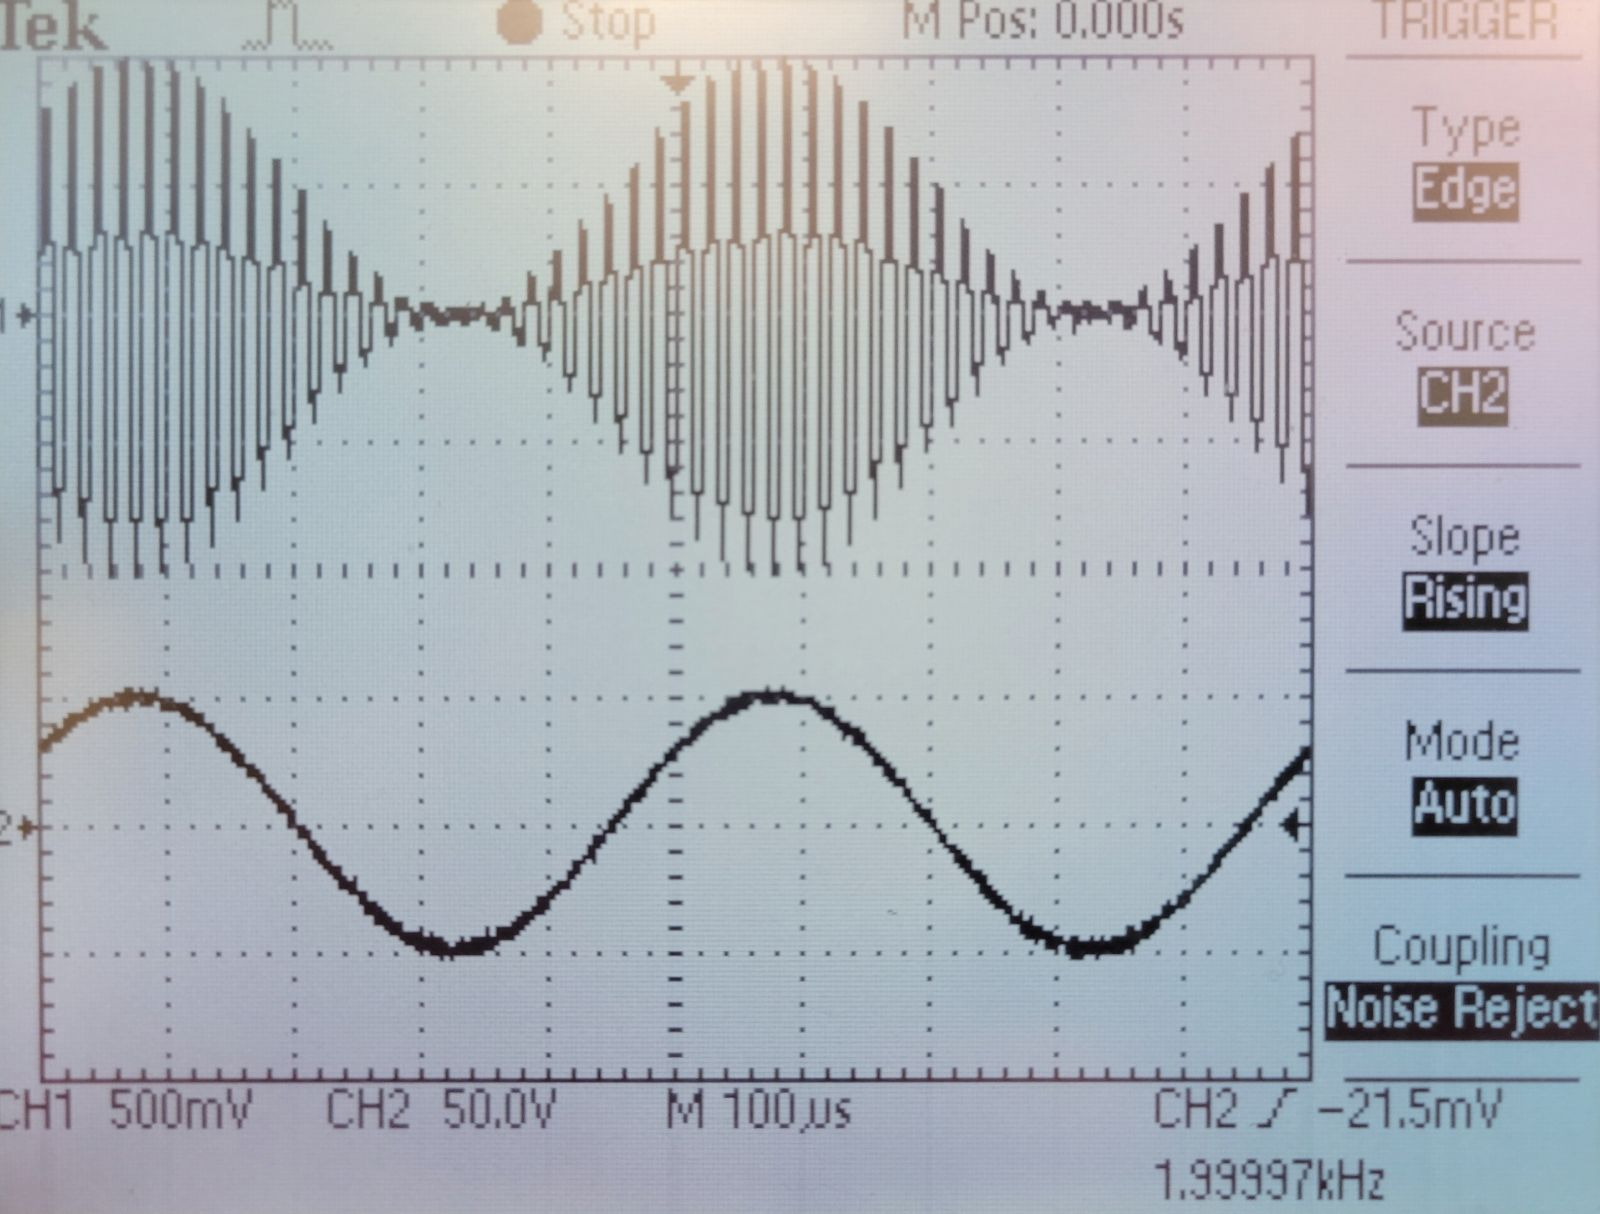
\includegraphics[width=0.45\textwidth]{fig2_1.png} & 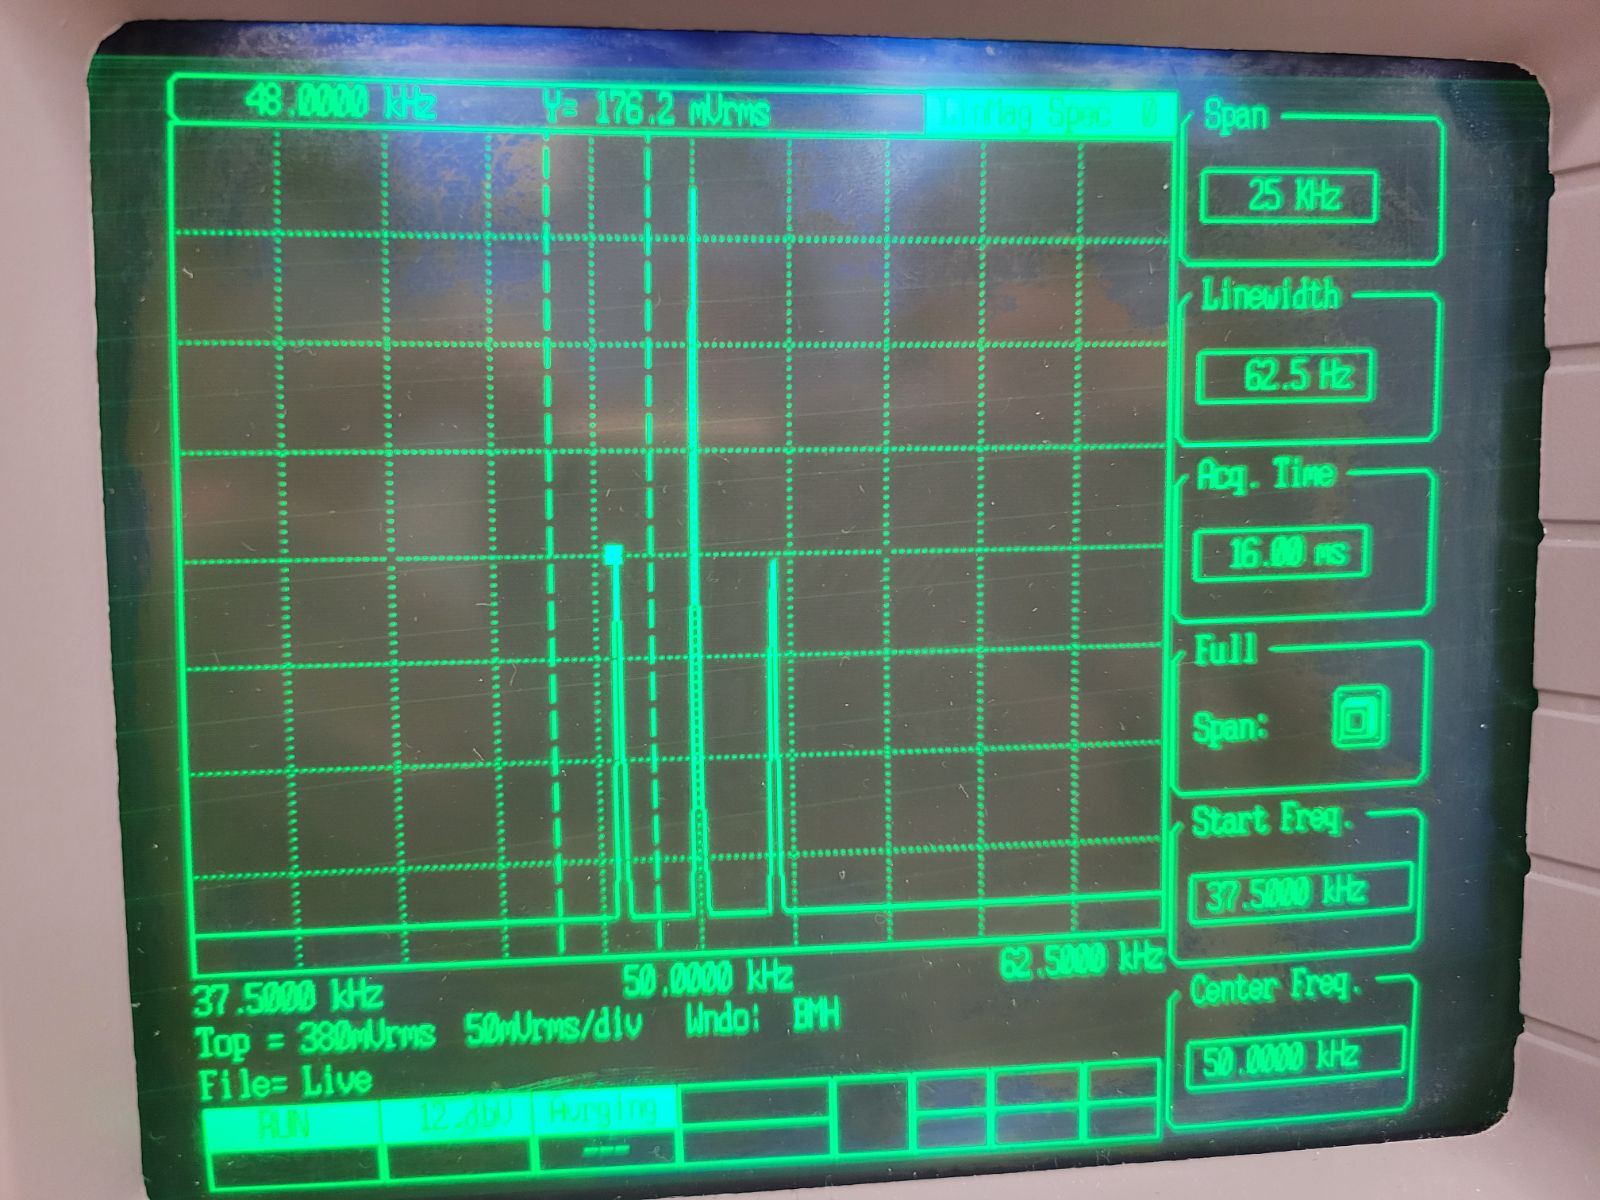
\includegraphics[width=0.45\textwidth]{fig2_2.png}
    \end{tabular}
    \captionsetup{width=0.8\textwidth}
    \caption{Scope (left) with bottom program content and 770 (right) view of AM Modulation of a 50 kHz carrier wave with a 2 kHz program wave.}
    \label{fig:am_modulation}
\end{figure*}

In Figure \ref{fig:am_modulation}, we see the scope and 770 view of the AM modulation of a 50 kHz carrier wave with a 2 kHz program wave.
The scope view shows familiar looking AM modulated waveform,
while the 770 clearly shows the carrier frequency at the center and the two sidebands which dictate the frequency of the program content.

\paragraph*{Changing content of the two waves}
\begin{itemize}
    \item Increase frequency of program content:
    \begin{itemize}
        \item The sidebands move further away from the carrier frequency just as the theory predicts $f_c \pm f_p$.
    \end{itemize}
    \item Change carrier frequency:
    \begin{itemize}
        \item Moves the 3 peak structure left or right (low freq and high freq respectively) on the 770 (Figure \ref{fig:2}).
        \item The envelope of the modulated waveform remains the same, but the inside oscillations increase as $f_c$ increases.
    \end{itemize}
    % fig2_3.png and fig2_4.png
    \begin{figure*}[ht]
        \centering
        \begin{tabular}{cc}
            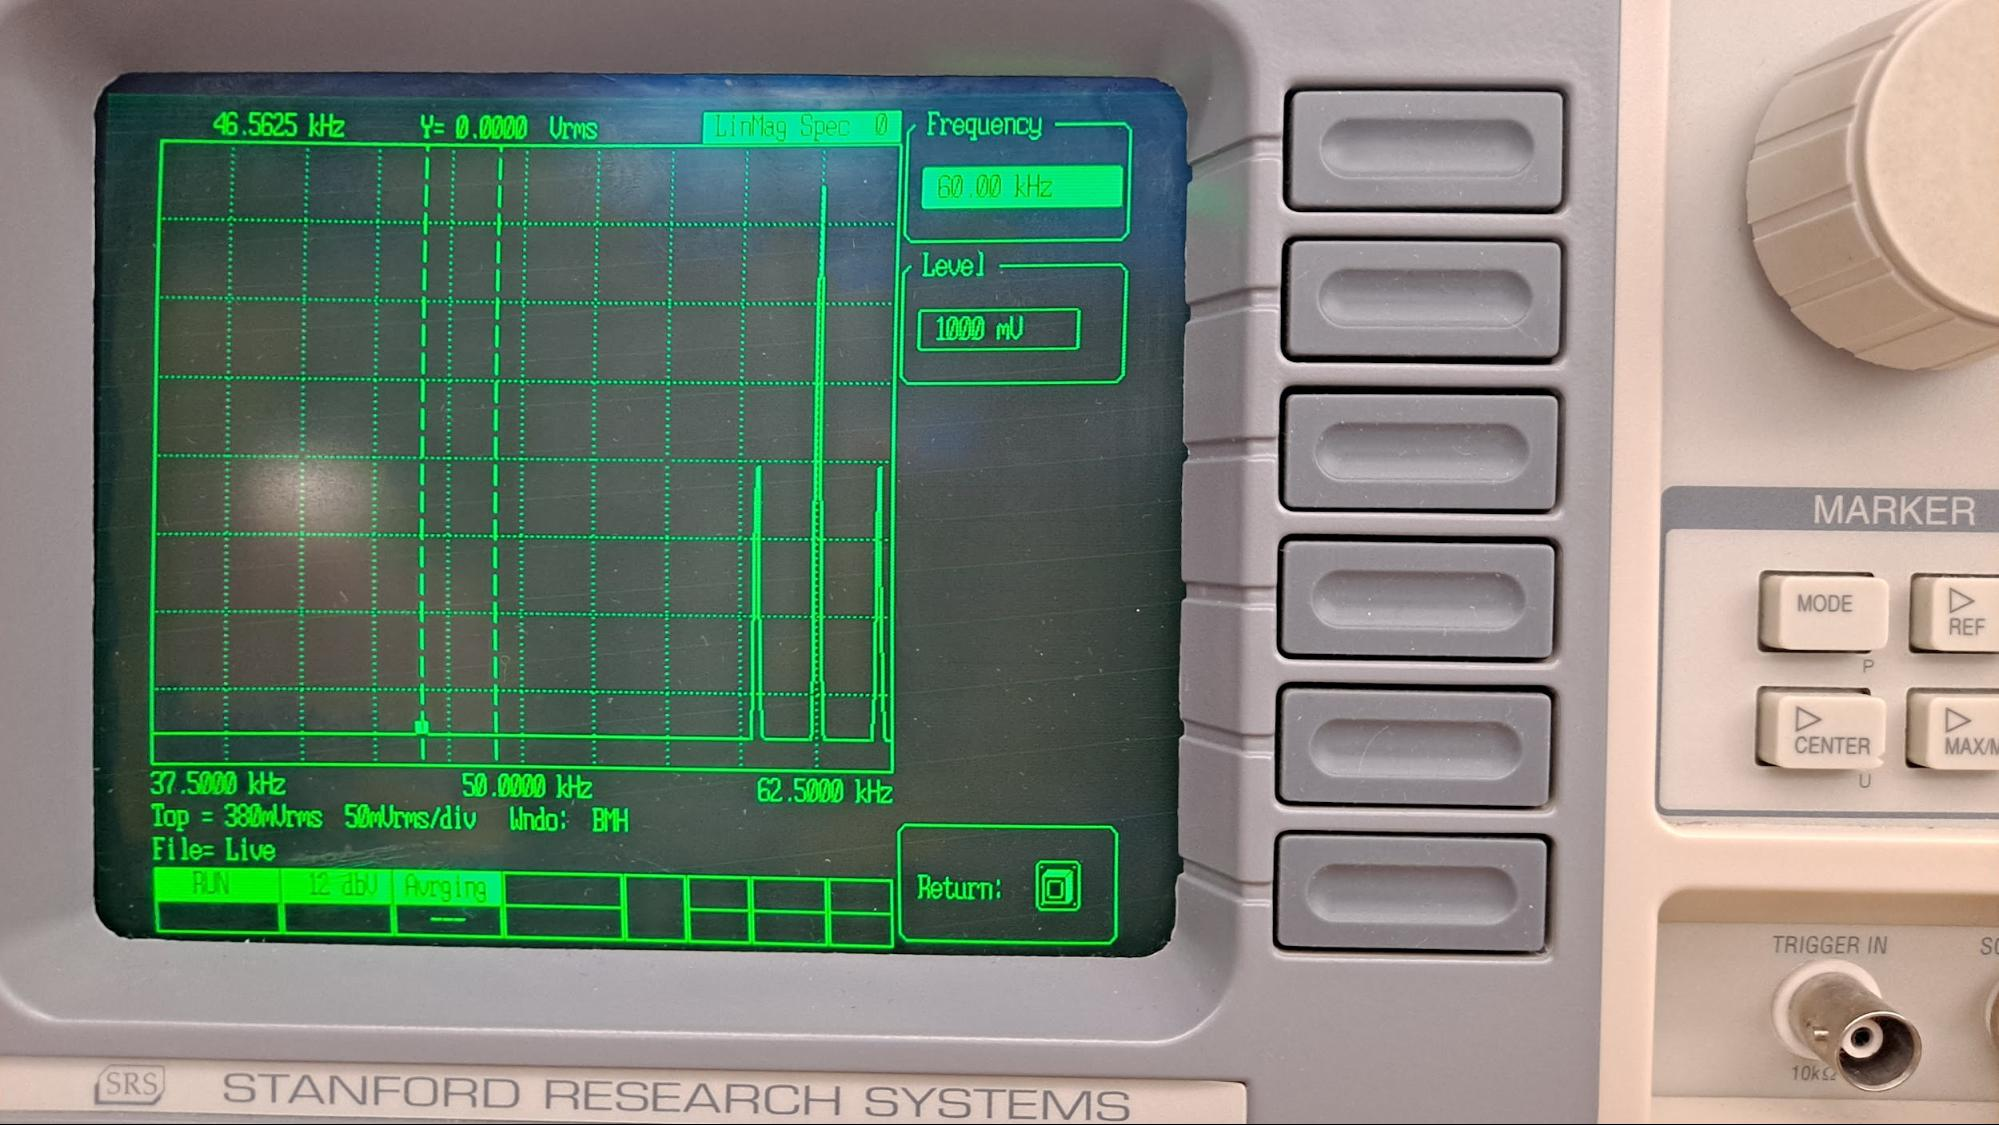
\includegraphics[width=0.45\textwidth]{fig2_3.png} & 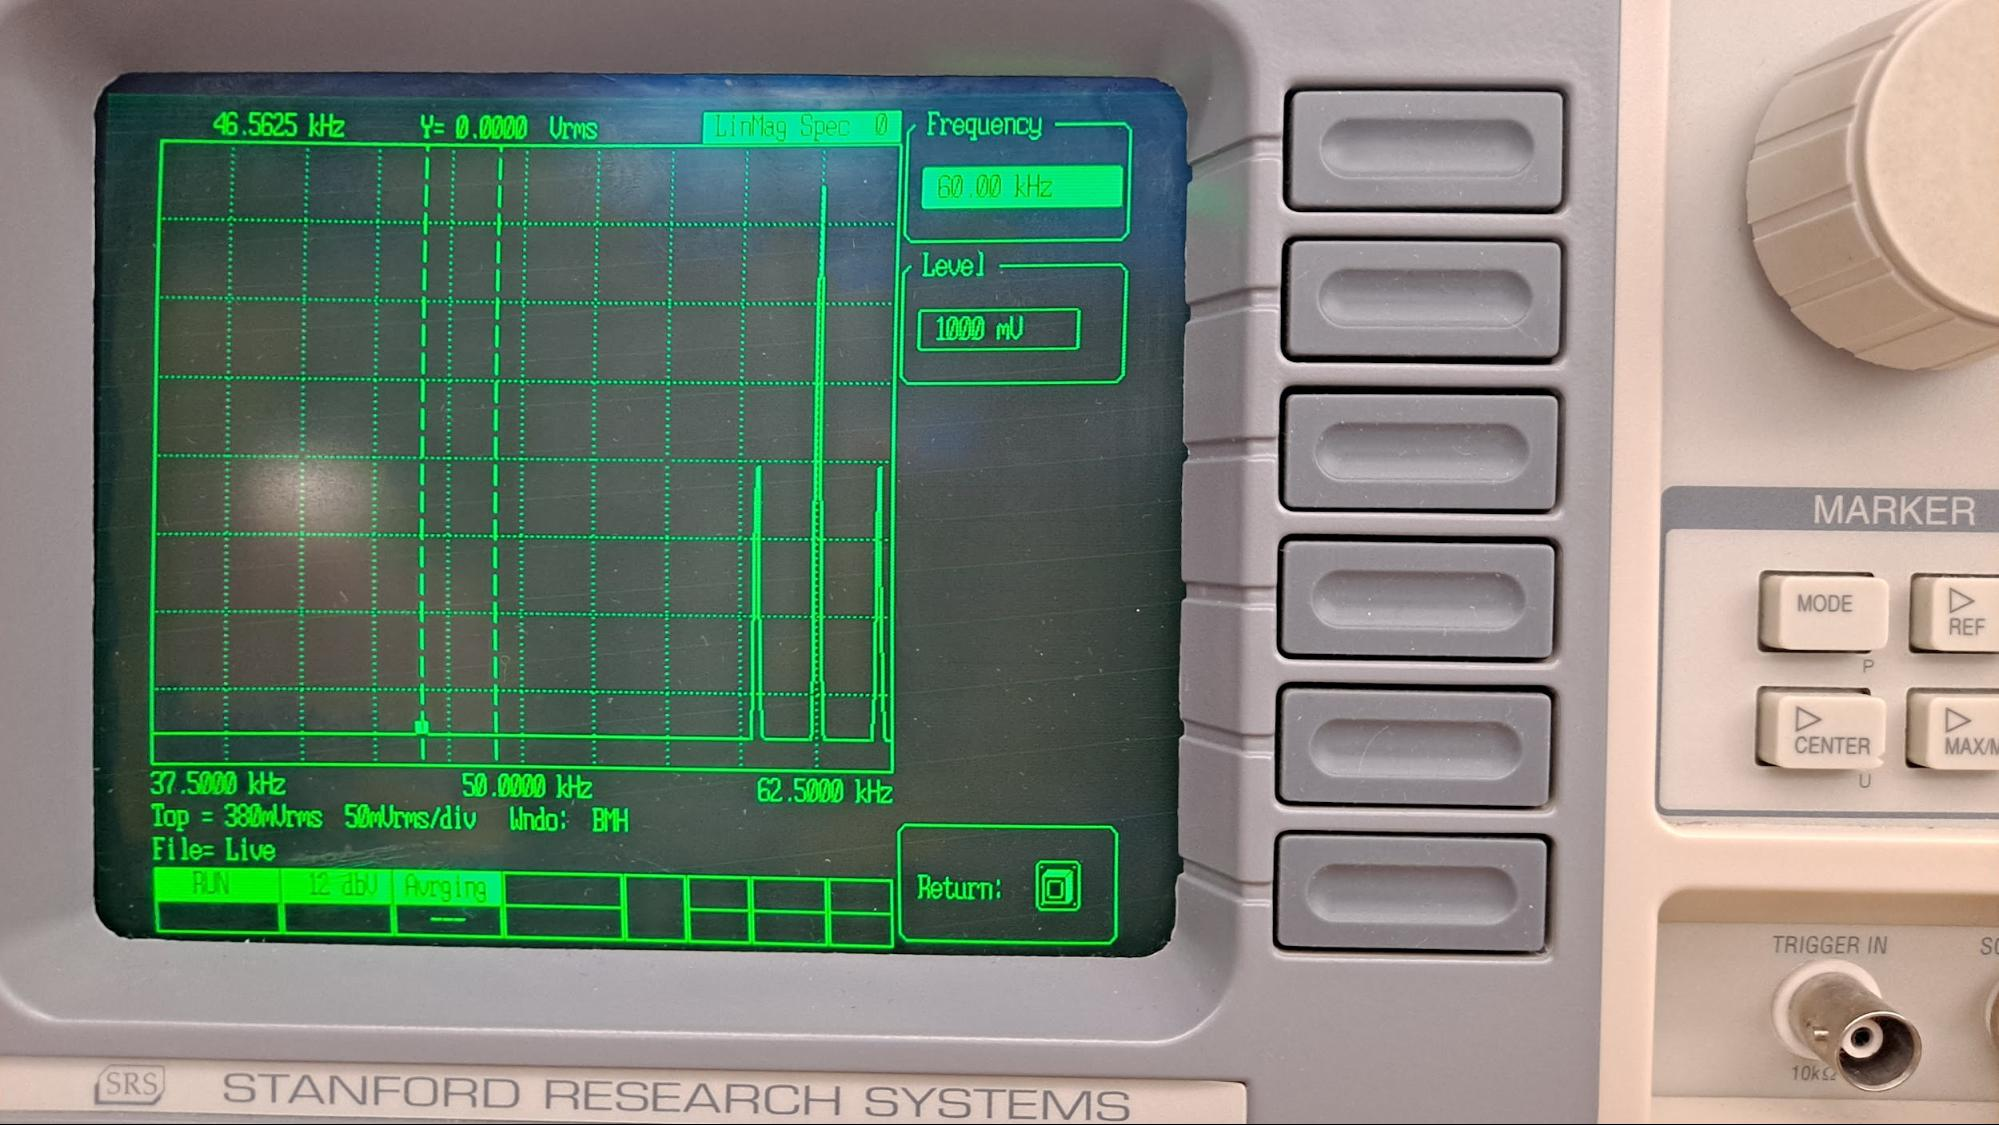
\includegraphics[width=0.45\textwidth]{fig2_4.png}
        \end{tabular}
        \captionsetup{width=0.8\textwidth}
        \caption{Increasing (right) and decreasing (left) program frequency.}
        \label{fig:2}
    \end{figure*}
    \item Program amplitude:
    \begin{itemize}
        \item Increasing the program amplitude increases the amplitude of the sidebands independent of the carrier amplitude (Fig. \ref{fig:3}).
    \end{itemize}
    % fig2_5.png
    \begin{figure}[ht]
        \centering
        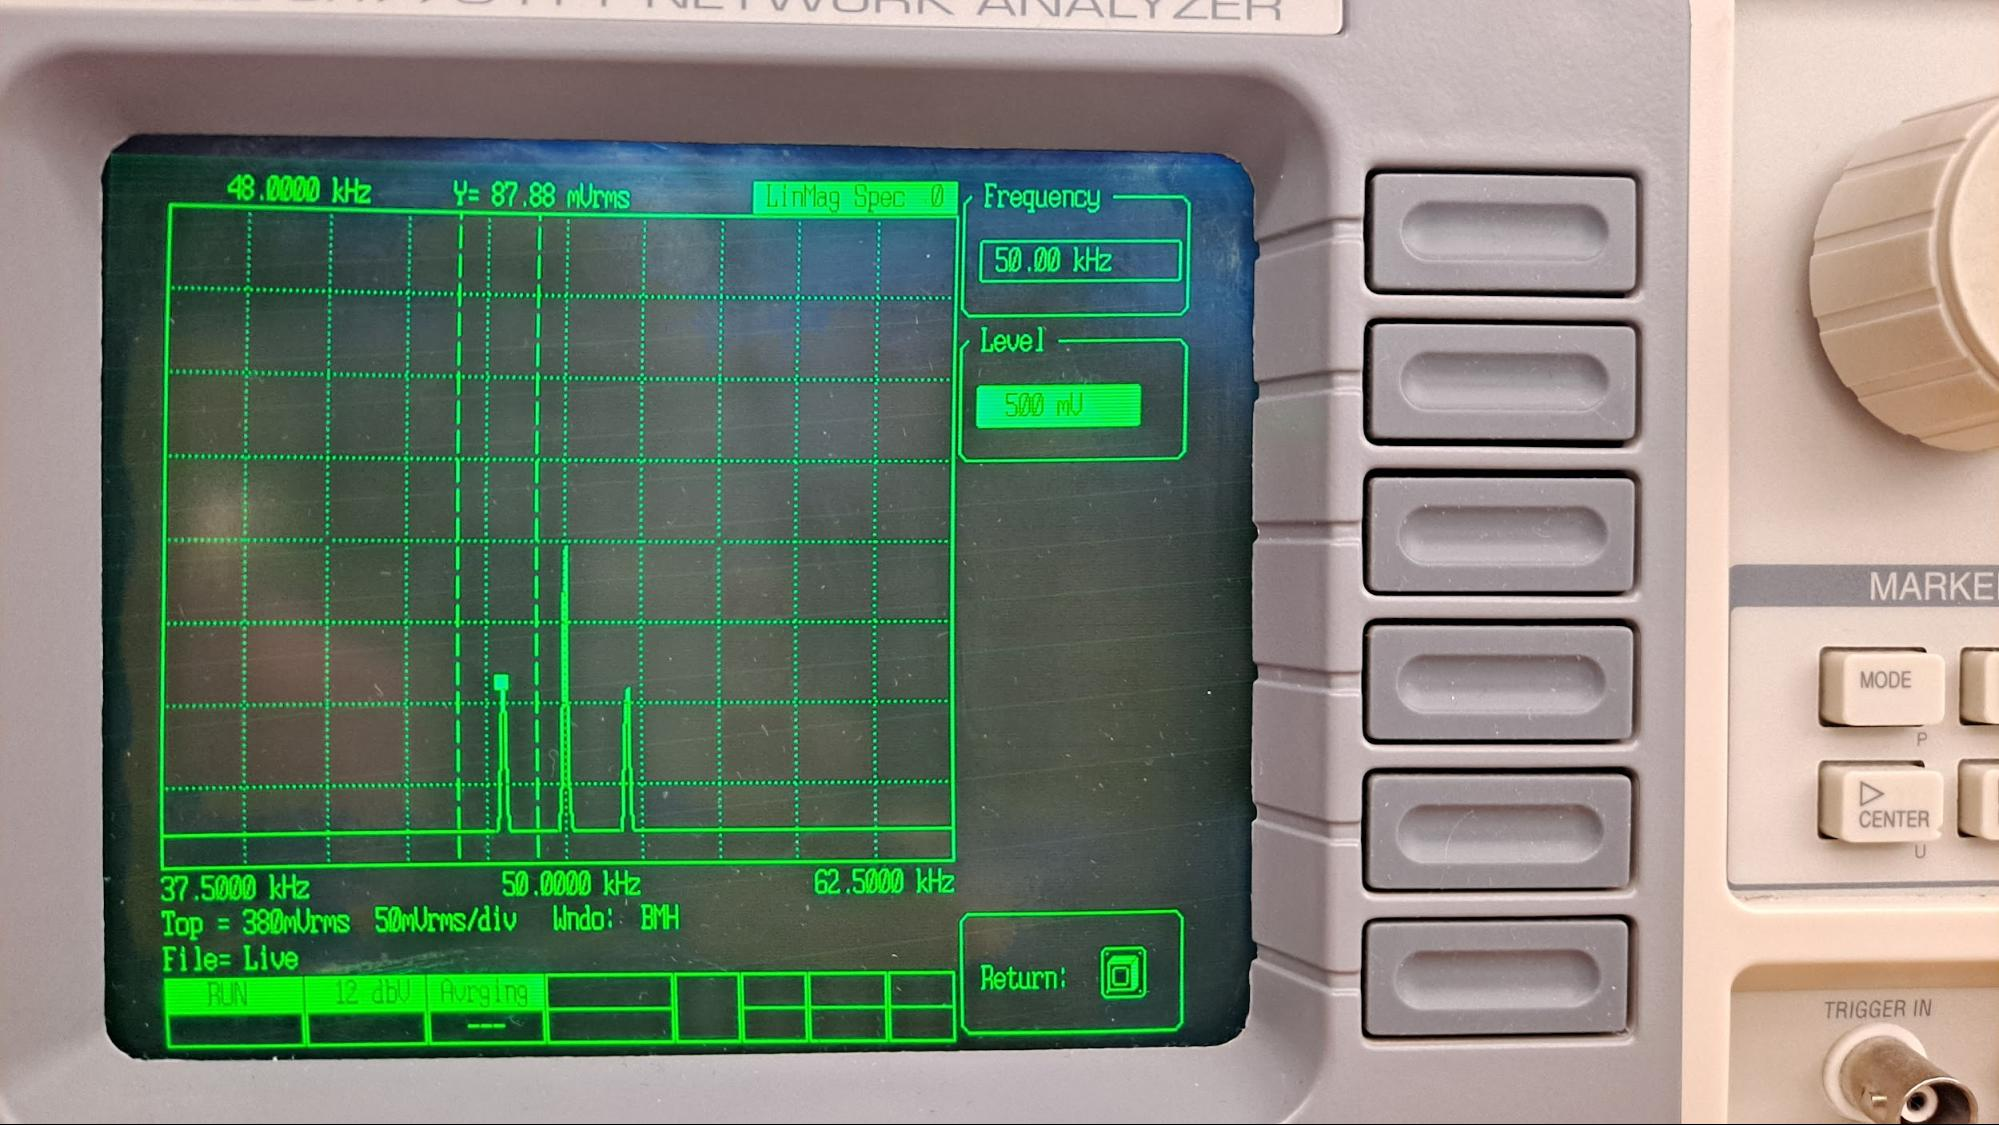
\includegraphics[width=0.45\textwidth]{fig2_5.png}
        \captionsetup{width=0.8\textwidth}
        \caption{Decreasing program amplitude.}
        \label{fig:3}
    \end{figure}
    \item Carrier amplitude:
    \begin{itemize}
        \item Increasing the carrier amplitude increases the amplitude of the carrier wave independent of the program amplitude (Fig. \ref{fig:4}).
    \end{itemize}
    % fig2_6.png and fig2_7.png
    \begin{figure*}[ht]
        \centering
        \begin{tabular}{cc}
            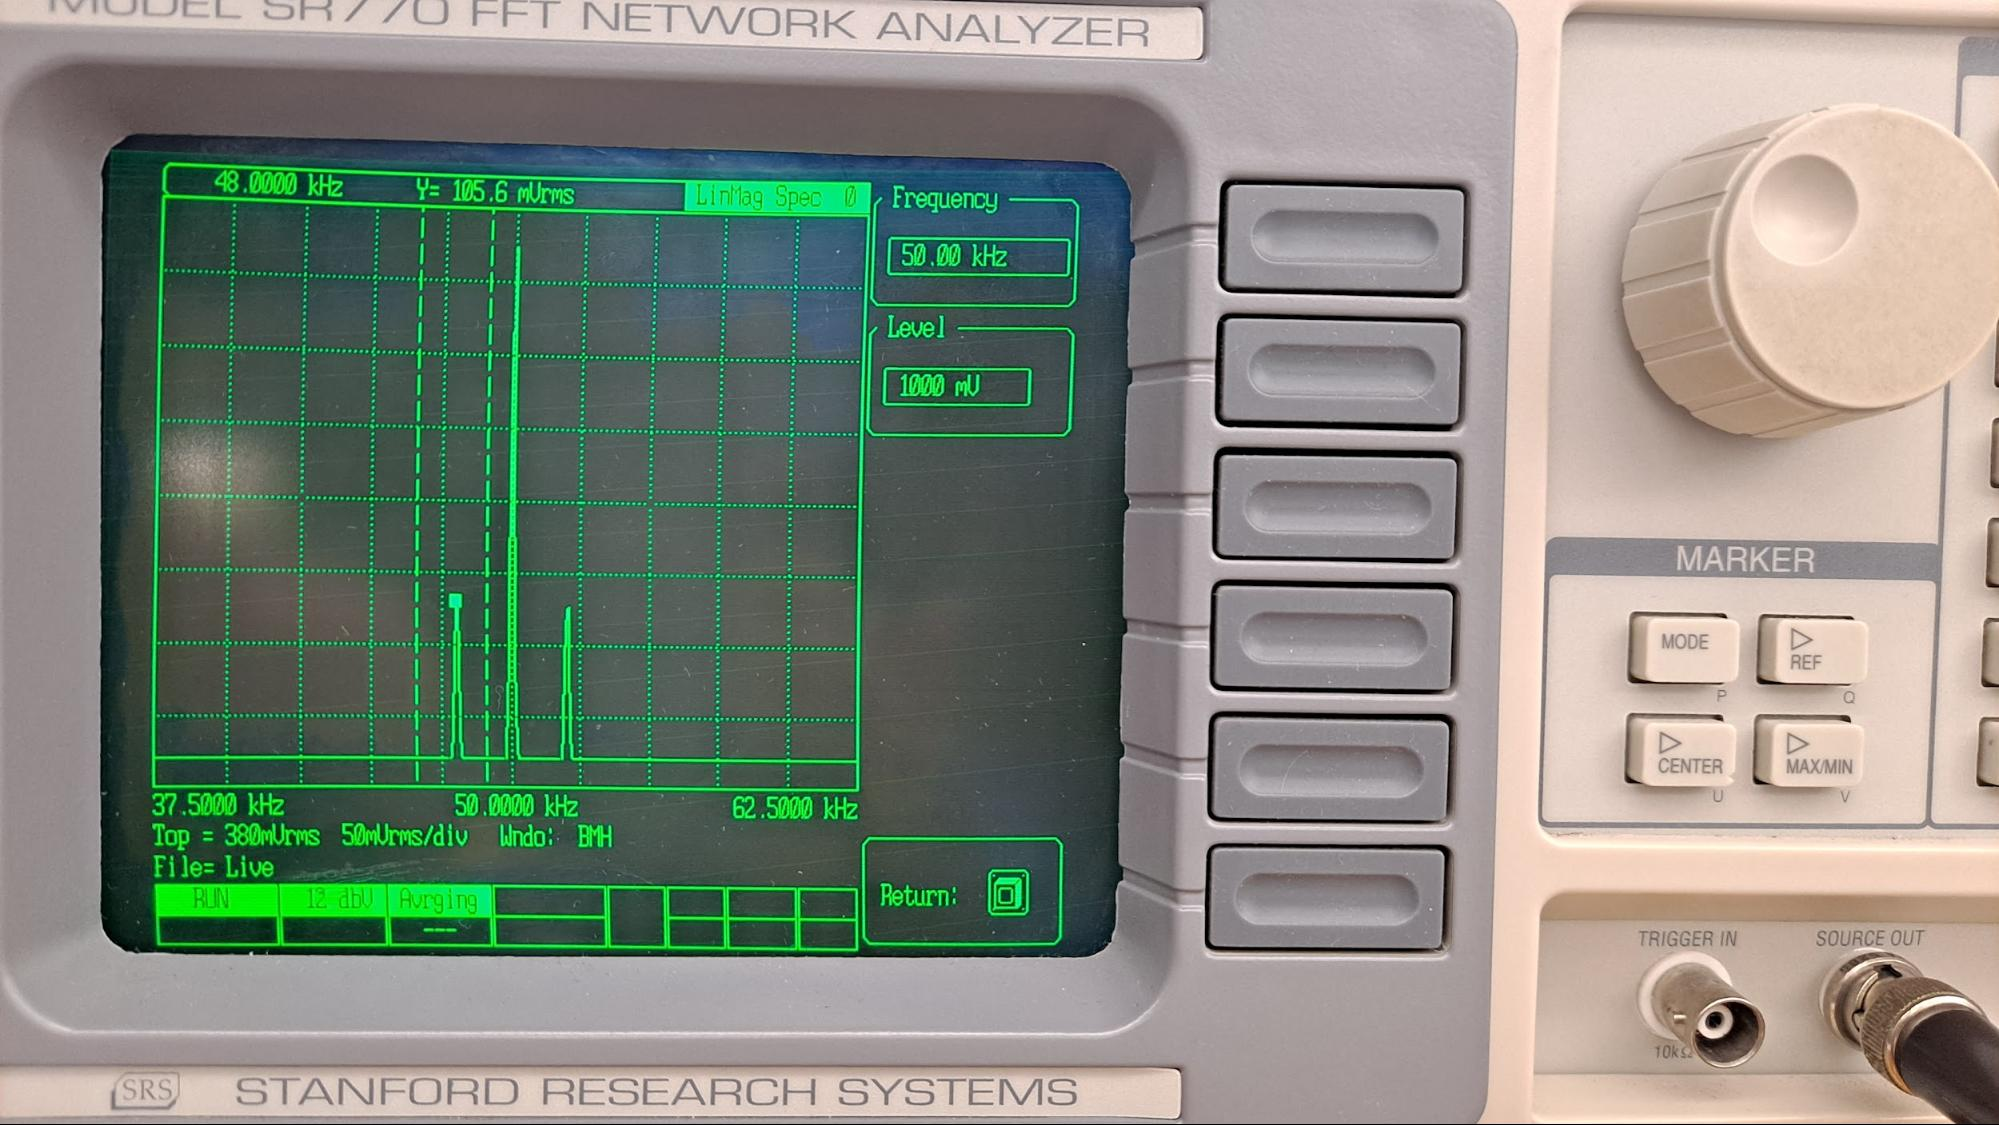
\includegraphics[width=0.45\textwidth]{fig2_6.png} & 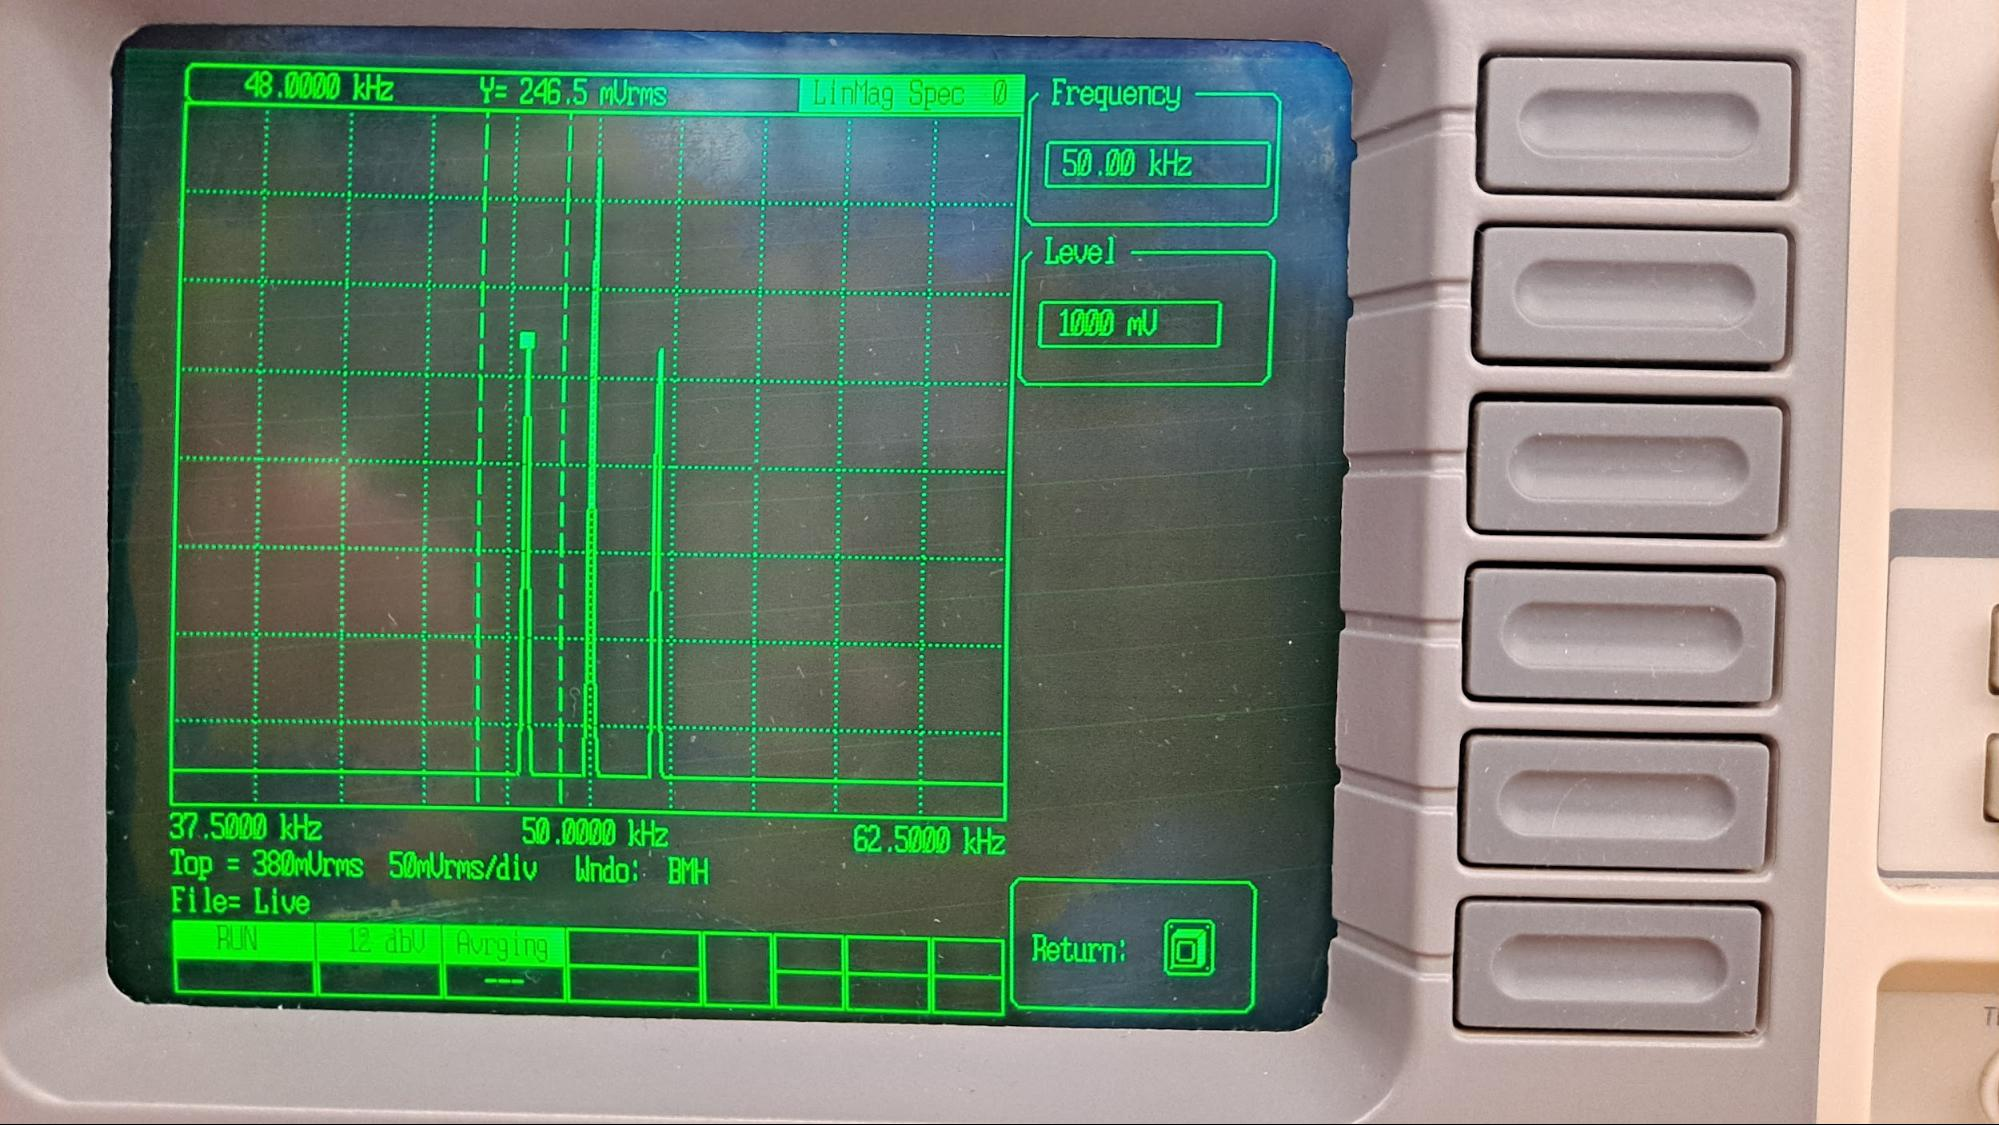
\includegraphics[width=0.45\textwidth]{fig2_7.png}
        \end{tabular}
        \captionsetup{width=0.8\textwidth}
        \caption{Increasing (right) and decreasing (left) carrier frequency.}
        \label{fig:4}
    \end{figure*}
    \item Program content to square wave:
    \begin{itemize}
        \item There are multiple sidebands at odd multiples of the program frequency.
    \end{itemize}
    % fig2_8.png and fig2_9.png
    \begin{figure*}[ht]
        \centering
        \begin{tabular}{cc}
            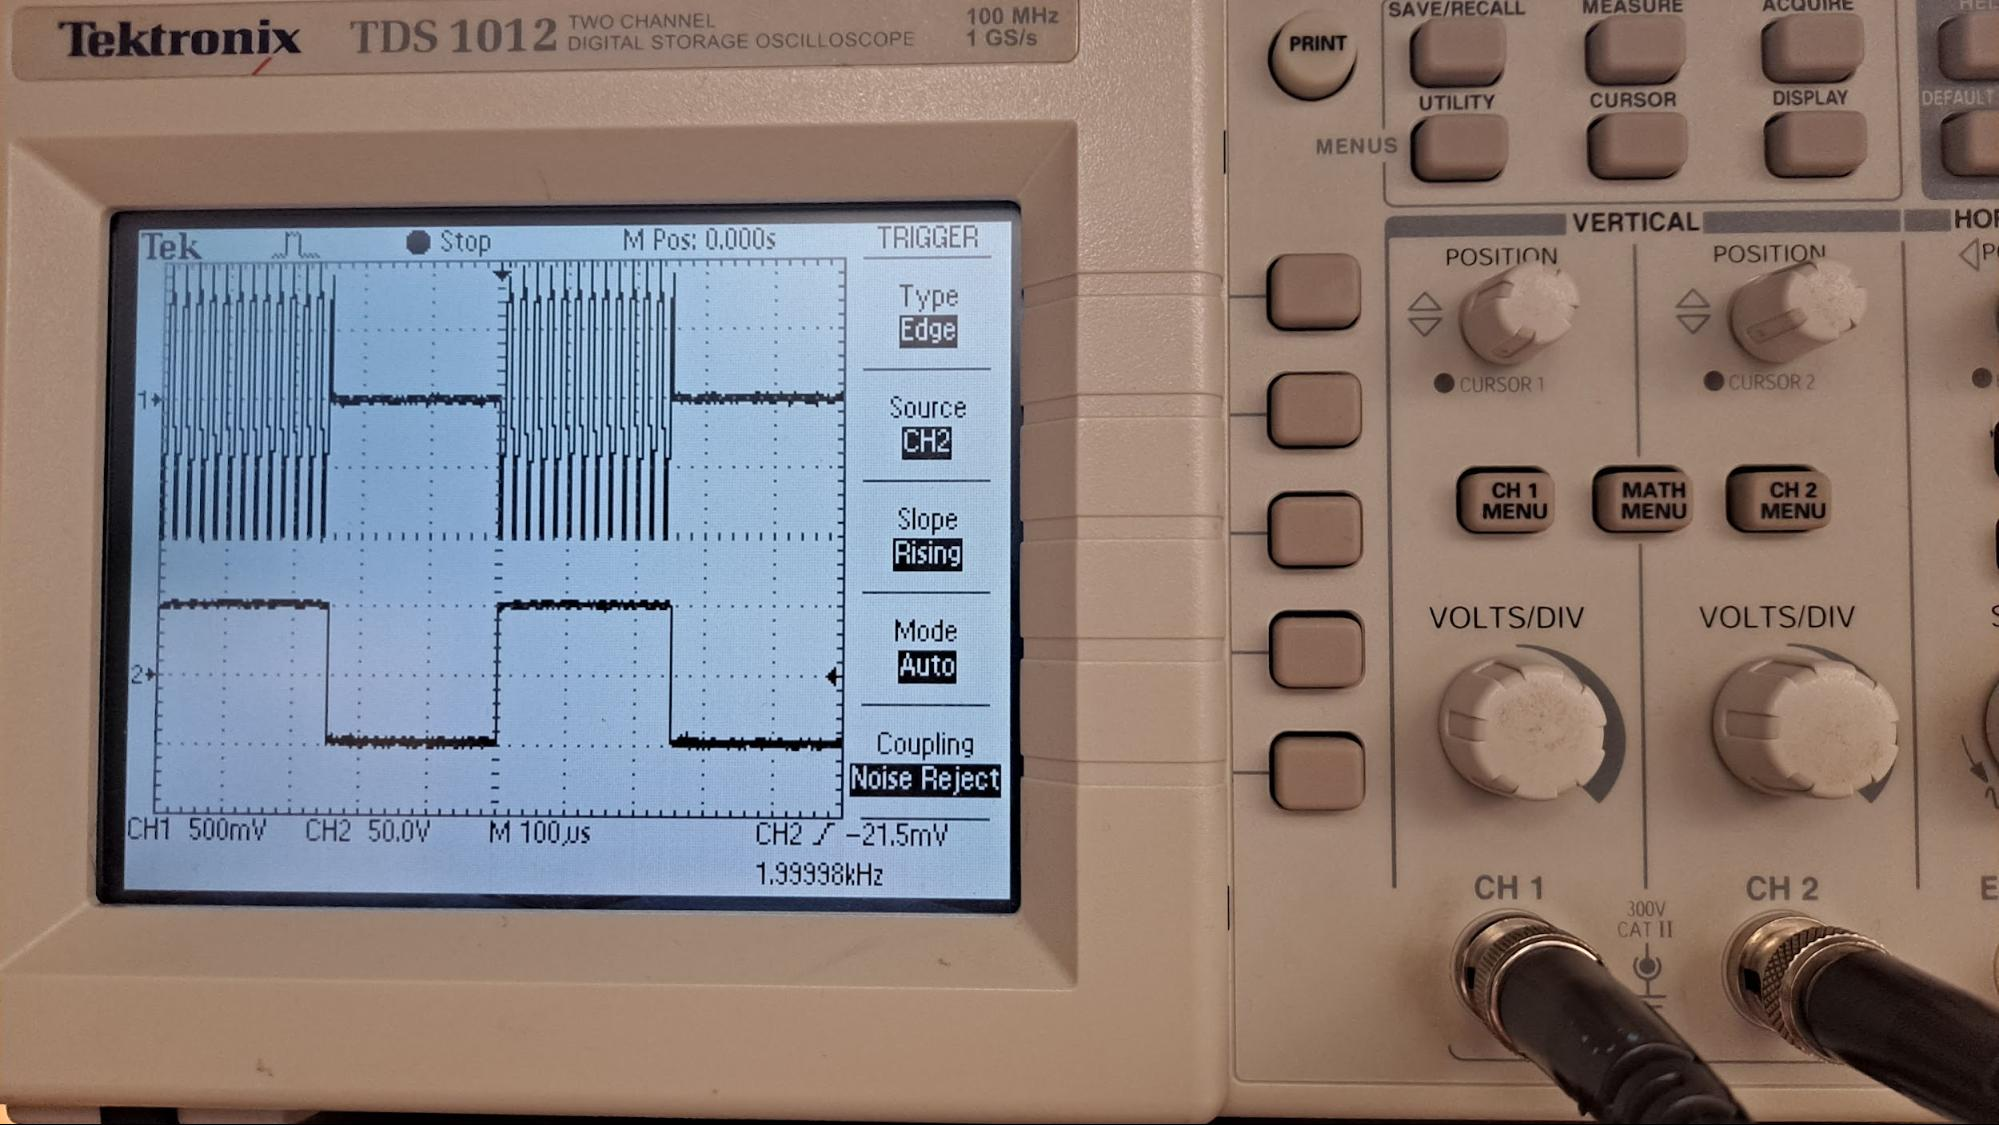
\includegraphics[width=0.45\textwidth]{fig2_8.png} & 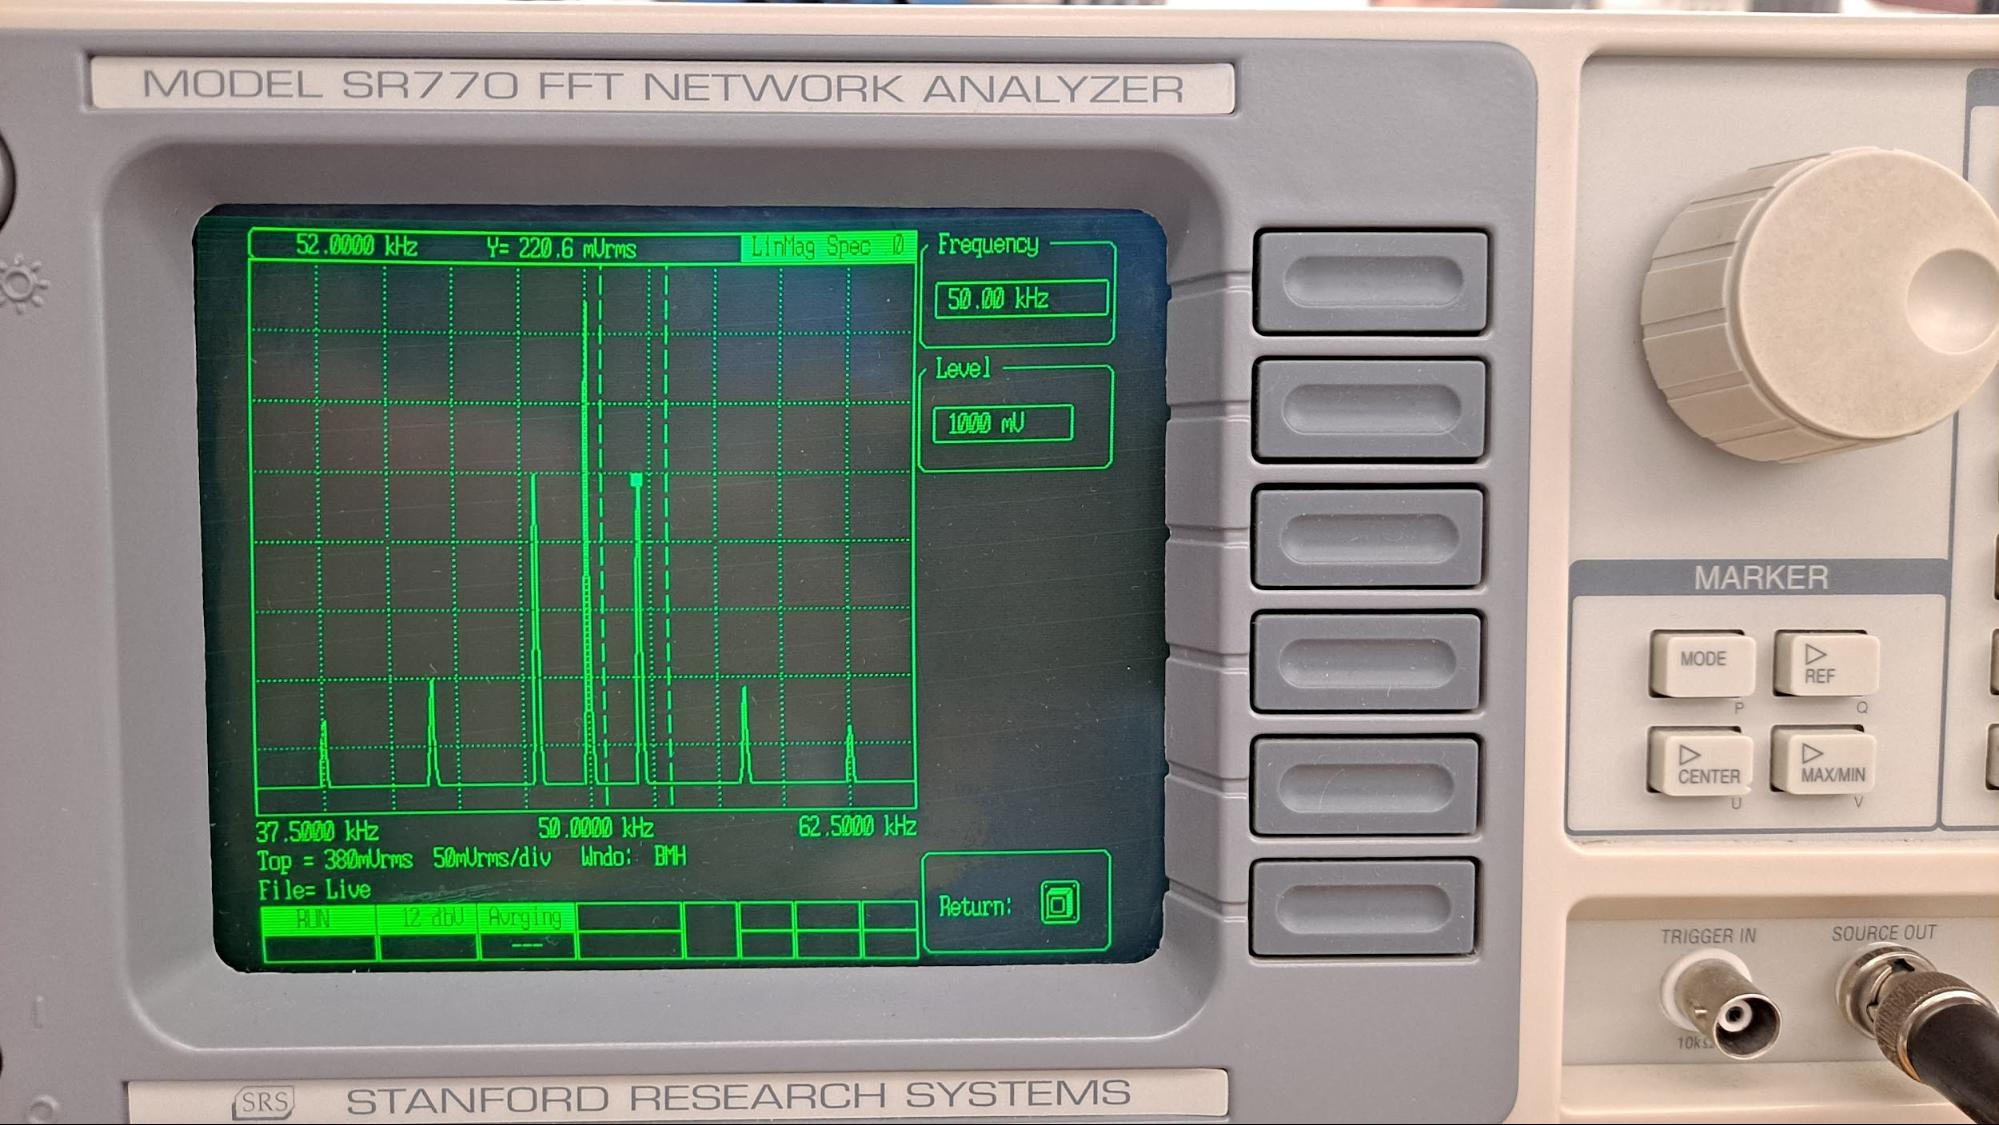
\includegraphics[width=0.45\textwidth]{fig2_9.png}
        \end{tabular}
        \captionsetup{width=0.8\textwidth}
        \caption{Scope (left) with program content in the bottom and 770 (right) view of AM Modulation of a 50 kHz carrier wave with a 2 kHz square wave program wave.}
        \label{fig:5}
    \end{figure*}
\end{itemize}

\paragraph*{Why $\alpha < 1$?}
The multiplier ouputs a scaled product of the two input signals
\begin{align*}
    V_{\text{out}} = \frac{V_A V_B}{10}
\end{align*}
for inputs with voltage $\pm 10$ V, and frequency lower than $1$ MHz. Thus for $5$ V DC input from the summer with the program signal gives
\begin{align*}
    V_{\text{out}} &= (5 V + P \cos(2\pi f_p t)) (A \cos(2\pi f_c t)) / 10 \\
    &= \frac{5A}{10} V \qt(1 + \frac{P}{5 V} \cos(2\pi f_p t)\qt) \cos(2\pi f_c t)
\end{align*}
So the waveform has a modulation index $\alpha = \frac{P}{5 V}$. In our first case (Fig. \ref{fig:am_modulation}), $P = 5 V$ so $\alpha = 1$,
Here the scope clearly shows the two distinct frequencies that make up the AM waveform---i.e., the envelope matches the program content shown simultaneously below,
and the carrier frequency is resolved in the small oscillations within the envelope.

When we increase $\alpha \to 2$ (Fig. ref here), the program content is overmodulated or \textit{distorted} which makes it hard to extract
out the program content from the modulated waveform. 


\subsection*{Chapter 11: AM Radio Reception}
\addcontentsline{toc}{subsection}{Chapter 11: AM Radio Reception}

\paragraph*{Notes}
\begin{itemize}
    \item Since AM radio signals are roughly 540-1600 kHz, i.e., 500-200 m wavelength, the EM waves are pretty uniform and can be received by our simple electrical wire antenna connected to an LC-resonant circuit. 
    \item The LC-resonant slighly tunes the frequency range into a narrow band of frequencies, which can be changed by adjusting the number of inductors we put in series (Fig. \ref{fig:5}).
    % fig2_11.png
    \begin{figure*}[ht]
        \centering
        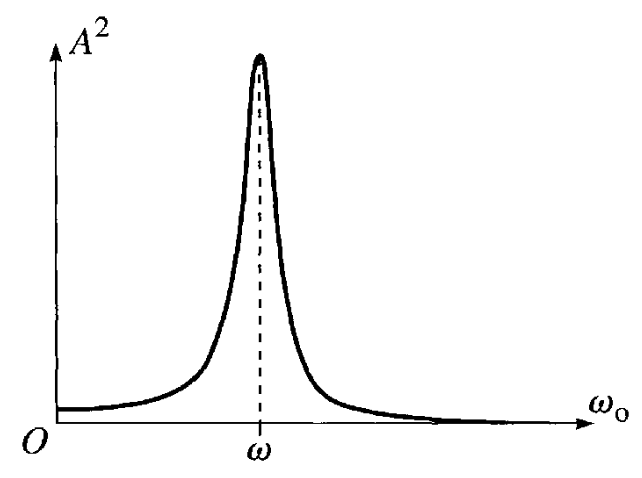
\includegraphics[width=0.45\textwidth]{fig2_11.png}
        \captionsetup{width=0.8\textwidth}
        \caption{Resonant frequency of RLC circuit (Taylor, Classical Mechanics). Our circuit has a broad resonance (rather than sharp) which will receive a band full of AM stations.}
        \label{fig:7}
    \end{figure*}
    \item Downcoversion: Before we narrow the frequency search range, we can first use downconversion to bring the high frequency AM signals to a lower frequency range provided by the High-Frequency (HF) Mixer module.
    \begin{itemize}
        \item Local-oscillator (LO) source: Using the 33500B, we set the LO frequency so that the difference between the LO and the AM signal is in the range of our 770 (100 kHz). 
        e.g., for target radio station (RF) $850$ kHz, setting the LO to $770$ or $930$ kHz will output a $80$ kHz difference frequency from the HF mixer. It will also ouput and sum \& difference frequencies from other radio stations which we must filter with the IF output.
        \item IF Filter: To create a fixed pass band that only allows the a narrow range of difference frequencies to pass through.
    \end{itemize}
    \item De-modulation: Turning AM signal into ``pure'' program content for the Audio Amp. \& Speak module.
    \begin{itemize}
        \item An AM signal waveform has a carrier $f_c$ carrying the program content $f_p$ in the sidebands $f_c \pm f_p$. 
        \item Tuning the LO frequency to $f_c$ will create a zero difference (or ``beat'') frequency thus the side bands of the IF are exactly the frequencies of the program content.
        e.g. for 850 kHz RF, set LO to 850 kHz and the Filter Freq. to 1 kHz. 
    \end{itemize}
    \item Heterodyne/Heterodyning: Shifting one frequency range to another
    \begin{itemize}
        \item Both Down-conversion and demodulating in this case are examples of heterodyning.
    \end{itemize}
\end{itemize}

% exp2_1.pdf and exp2_2.pdf
\begin{figure*}[ht]
    \centering
    \begin{tabular}{cc}
        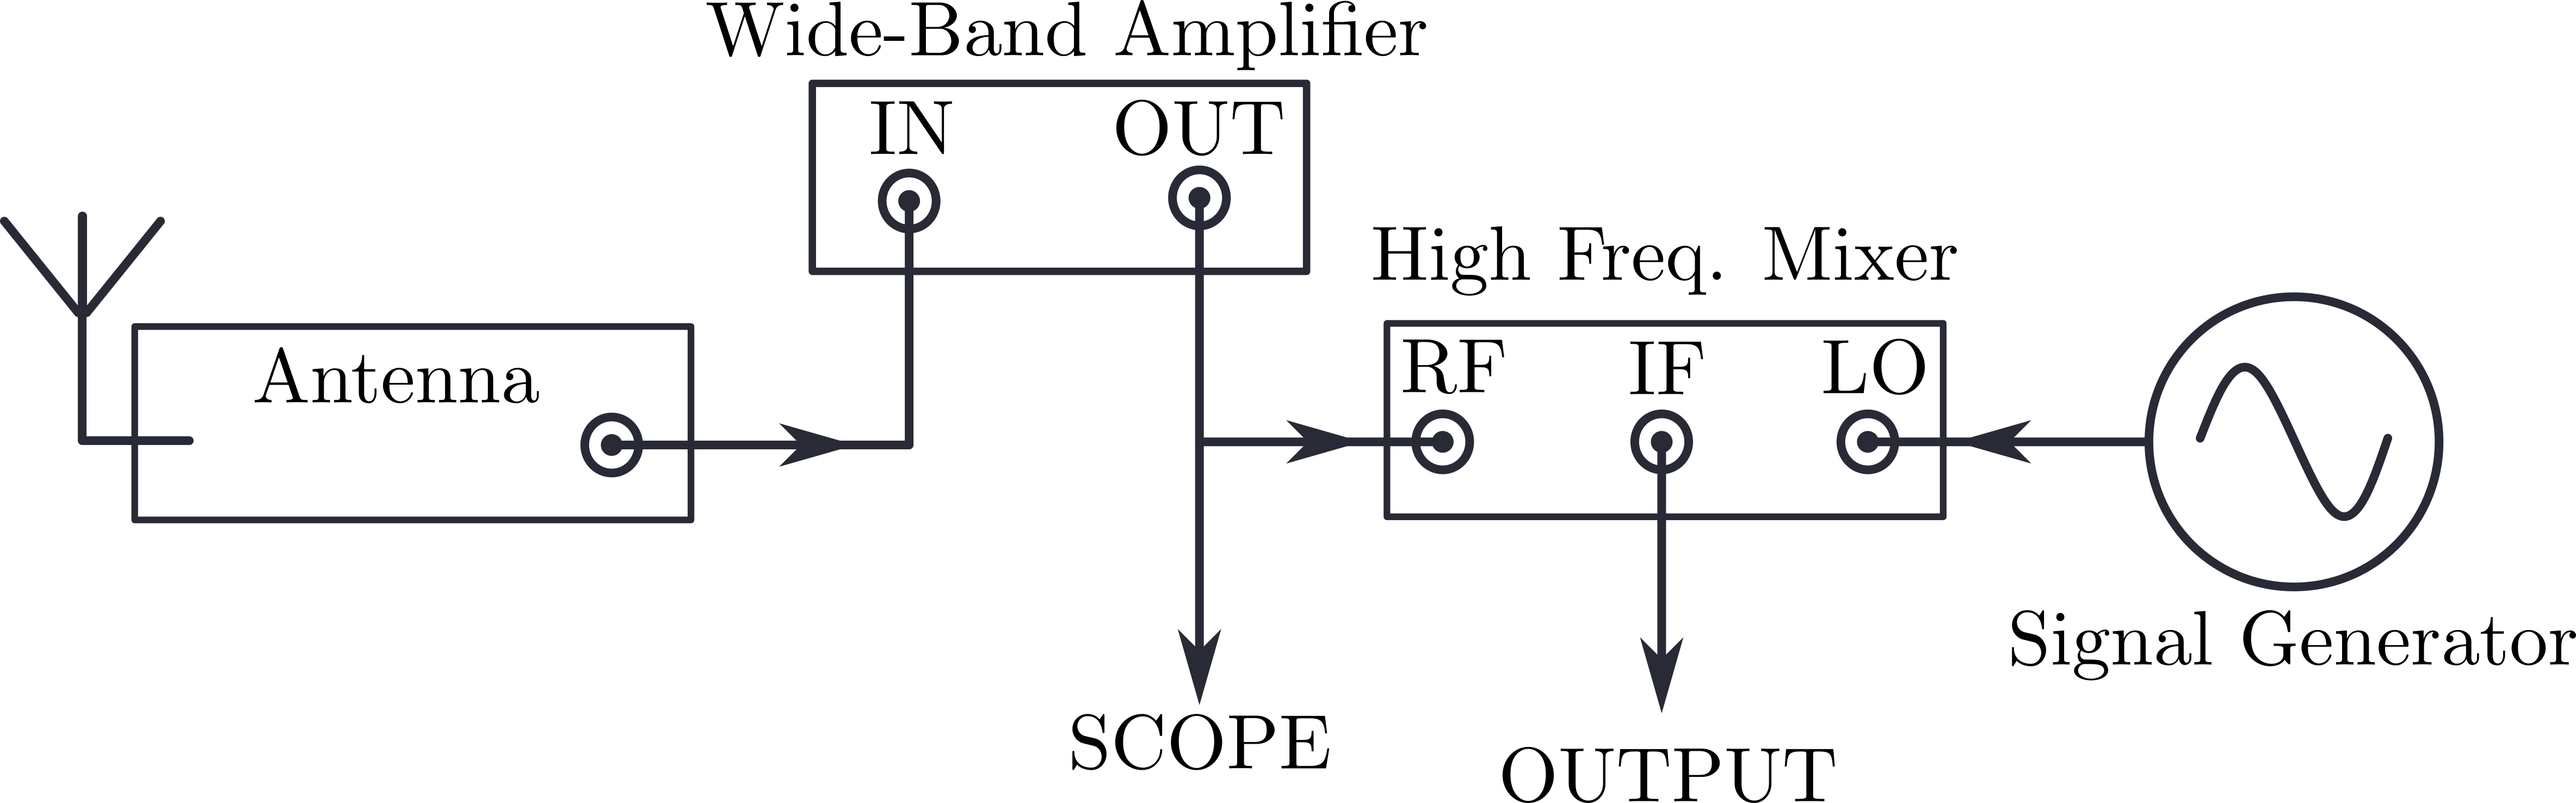
\includegraphics[width=0.45\textwidth]{exp2_1.png} & 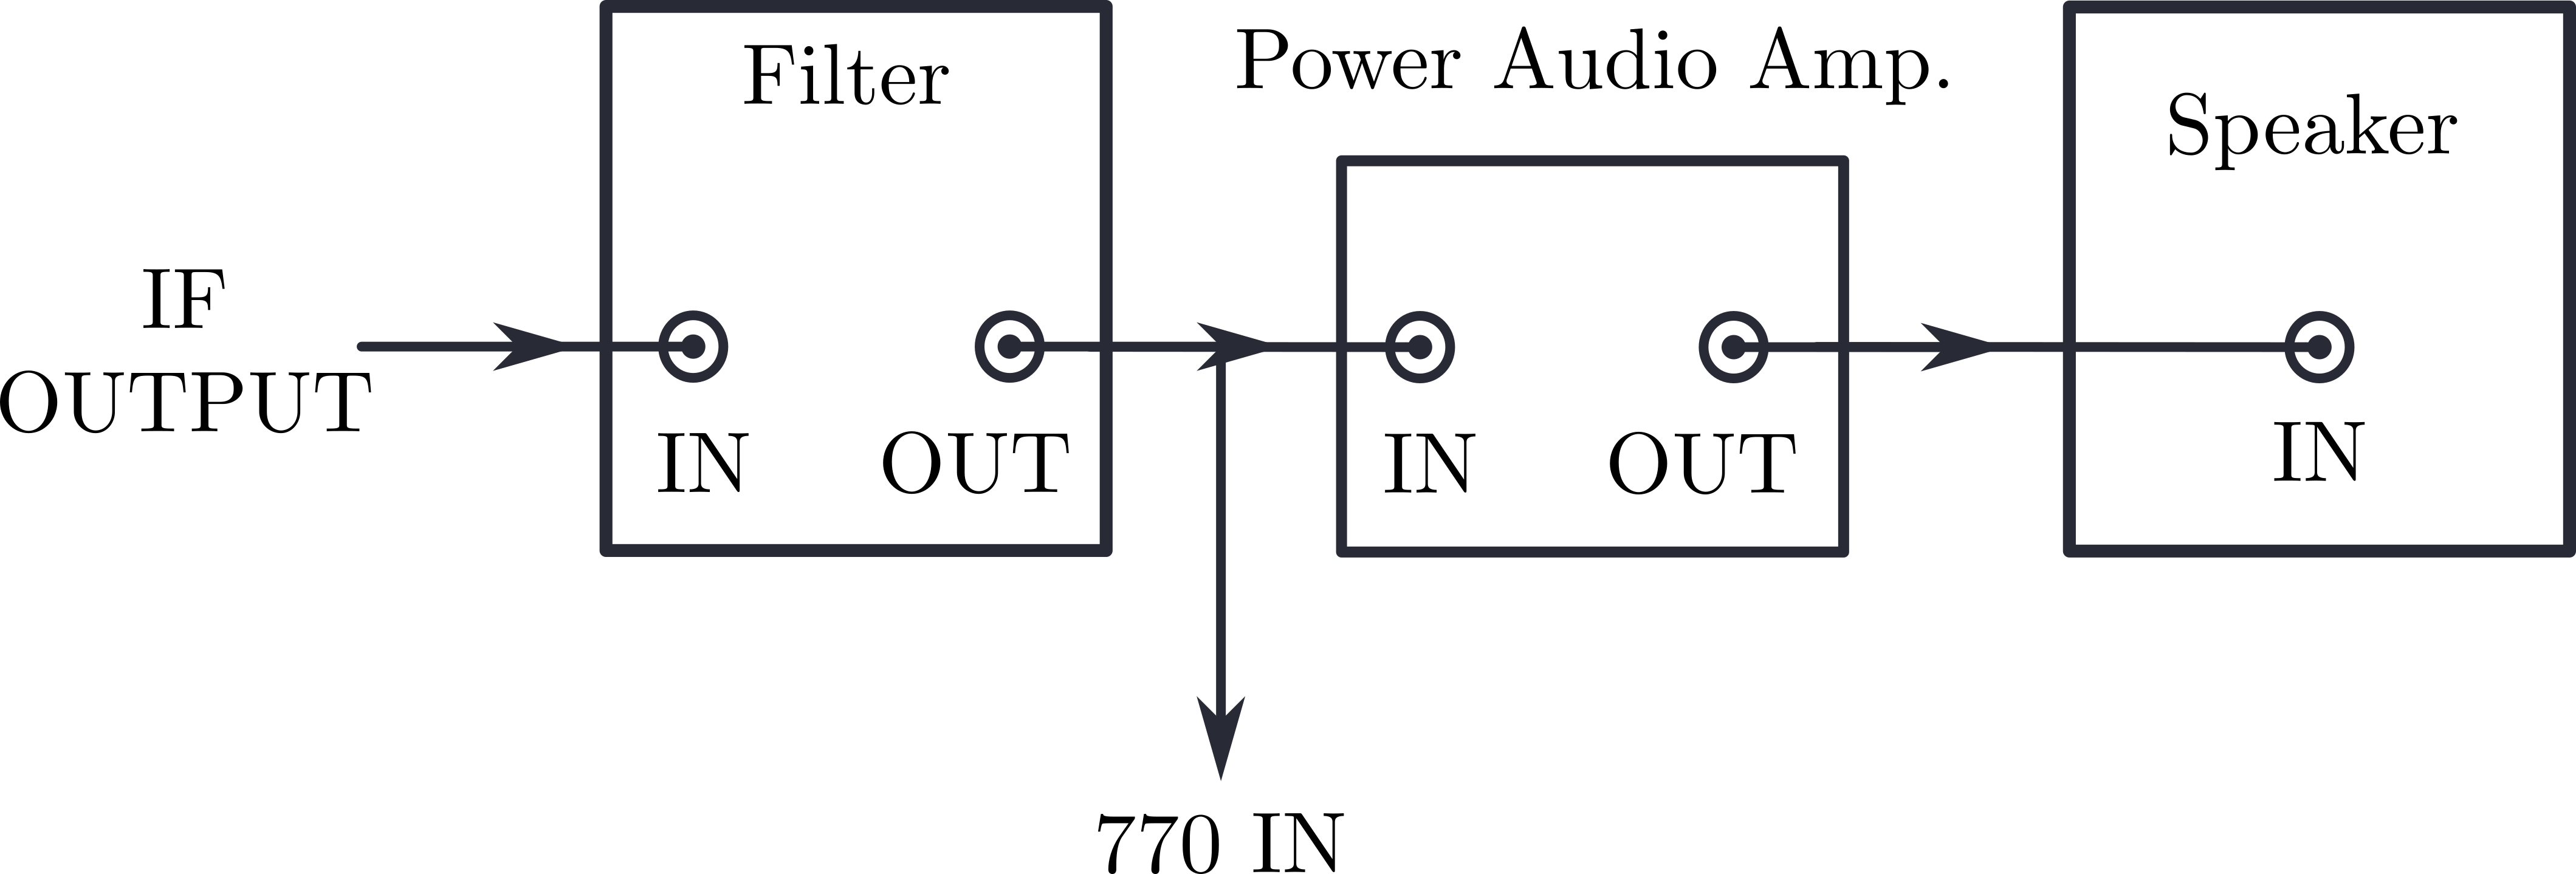
\includegraphics[width=0.45\textwidth]{exp2_2.png}
    \end{tabular}
    \captionsetup{width=0.8\textwidth}
    \caption{Experimental setup for AM radio reception.}
    \label{fig:6}
\end{figure*}

\paragraph*{Experiment:} Finding Radio Stations 
\begin{itemize}
    \item First note a near by radio station we can pick up from St. Louis \href{https://radio-locator.com/cgi-bin/locate?select=city&city=saint+louis&state=mo&x=0&y=0}{(Radio Station List)}. e.g. KFUO $f_{RF} = 850$ kHz.
    \item Set three inductors in series on the radio antenna circuit (more inductors in series add more inductance and decrease the resonant frequency).
    \item Radio antenna circuit OUPUT $\to$ Wideband Amp  $1\times 1 \times 10$ (10x) or until the signal is visible on the scope
    \item Wideband Amp OUTPUT $\to$ HF Mixer INPUT RF \& scope
    \item 33500B 1 V and Freq. 770 kHz (80 kHz differnce freq.) OUTPUT $\to$ HF Mixer (Down-conversion) INPUT LO 
    \item IF OUT $\to$ Filter Module 80 kHz; 8 Gain; Band-pass
    \item Filter OUT $\to$ Power Audio Amp. (Adjust gain until you hear noise or signal) \& 770 (LOG magnitude, MEASure Spectrum, and Averaging 16 to reduce noise and to have a fast response to the signal) and and note the visualized signal
    \item Power Audio Amp. OUT $\to$ Speaker Module
    \item Tune the LO frequency to get a strong signal using multiple difference frequency combinations, i.e., For 850 kHz RF, set LO to 930 kHz.
    \item De-modulate the signal by tuning the LO frequency \textit{exactly} to the Radio station frequency (carrier freq), i.e., the zero beat frequency—--e.g. For 850 kHz (KFUO) Radio Station, tune the LO to 850 kHz, the Filter Freq. to 1 or 3 kHz and decrease $Q \to 0.71$
\end{itemize}

\paragraph*{Observations} 
\begin{figure*}[ht]
    \centering
    \begin{minipage}{0.45\textwidth}
        \centering
        \includegraphics[width=\textwidth, page=2]{fig2_12.pdf}
        \caption{TDS 1012 oscilloscope view}
        \label{fig:2.12}
    \end{minipage}\hfill
    \begin{minipage}{0.45\textwidth}
        \centering
        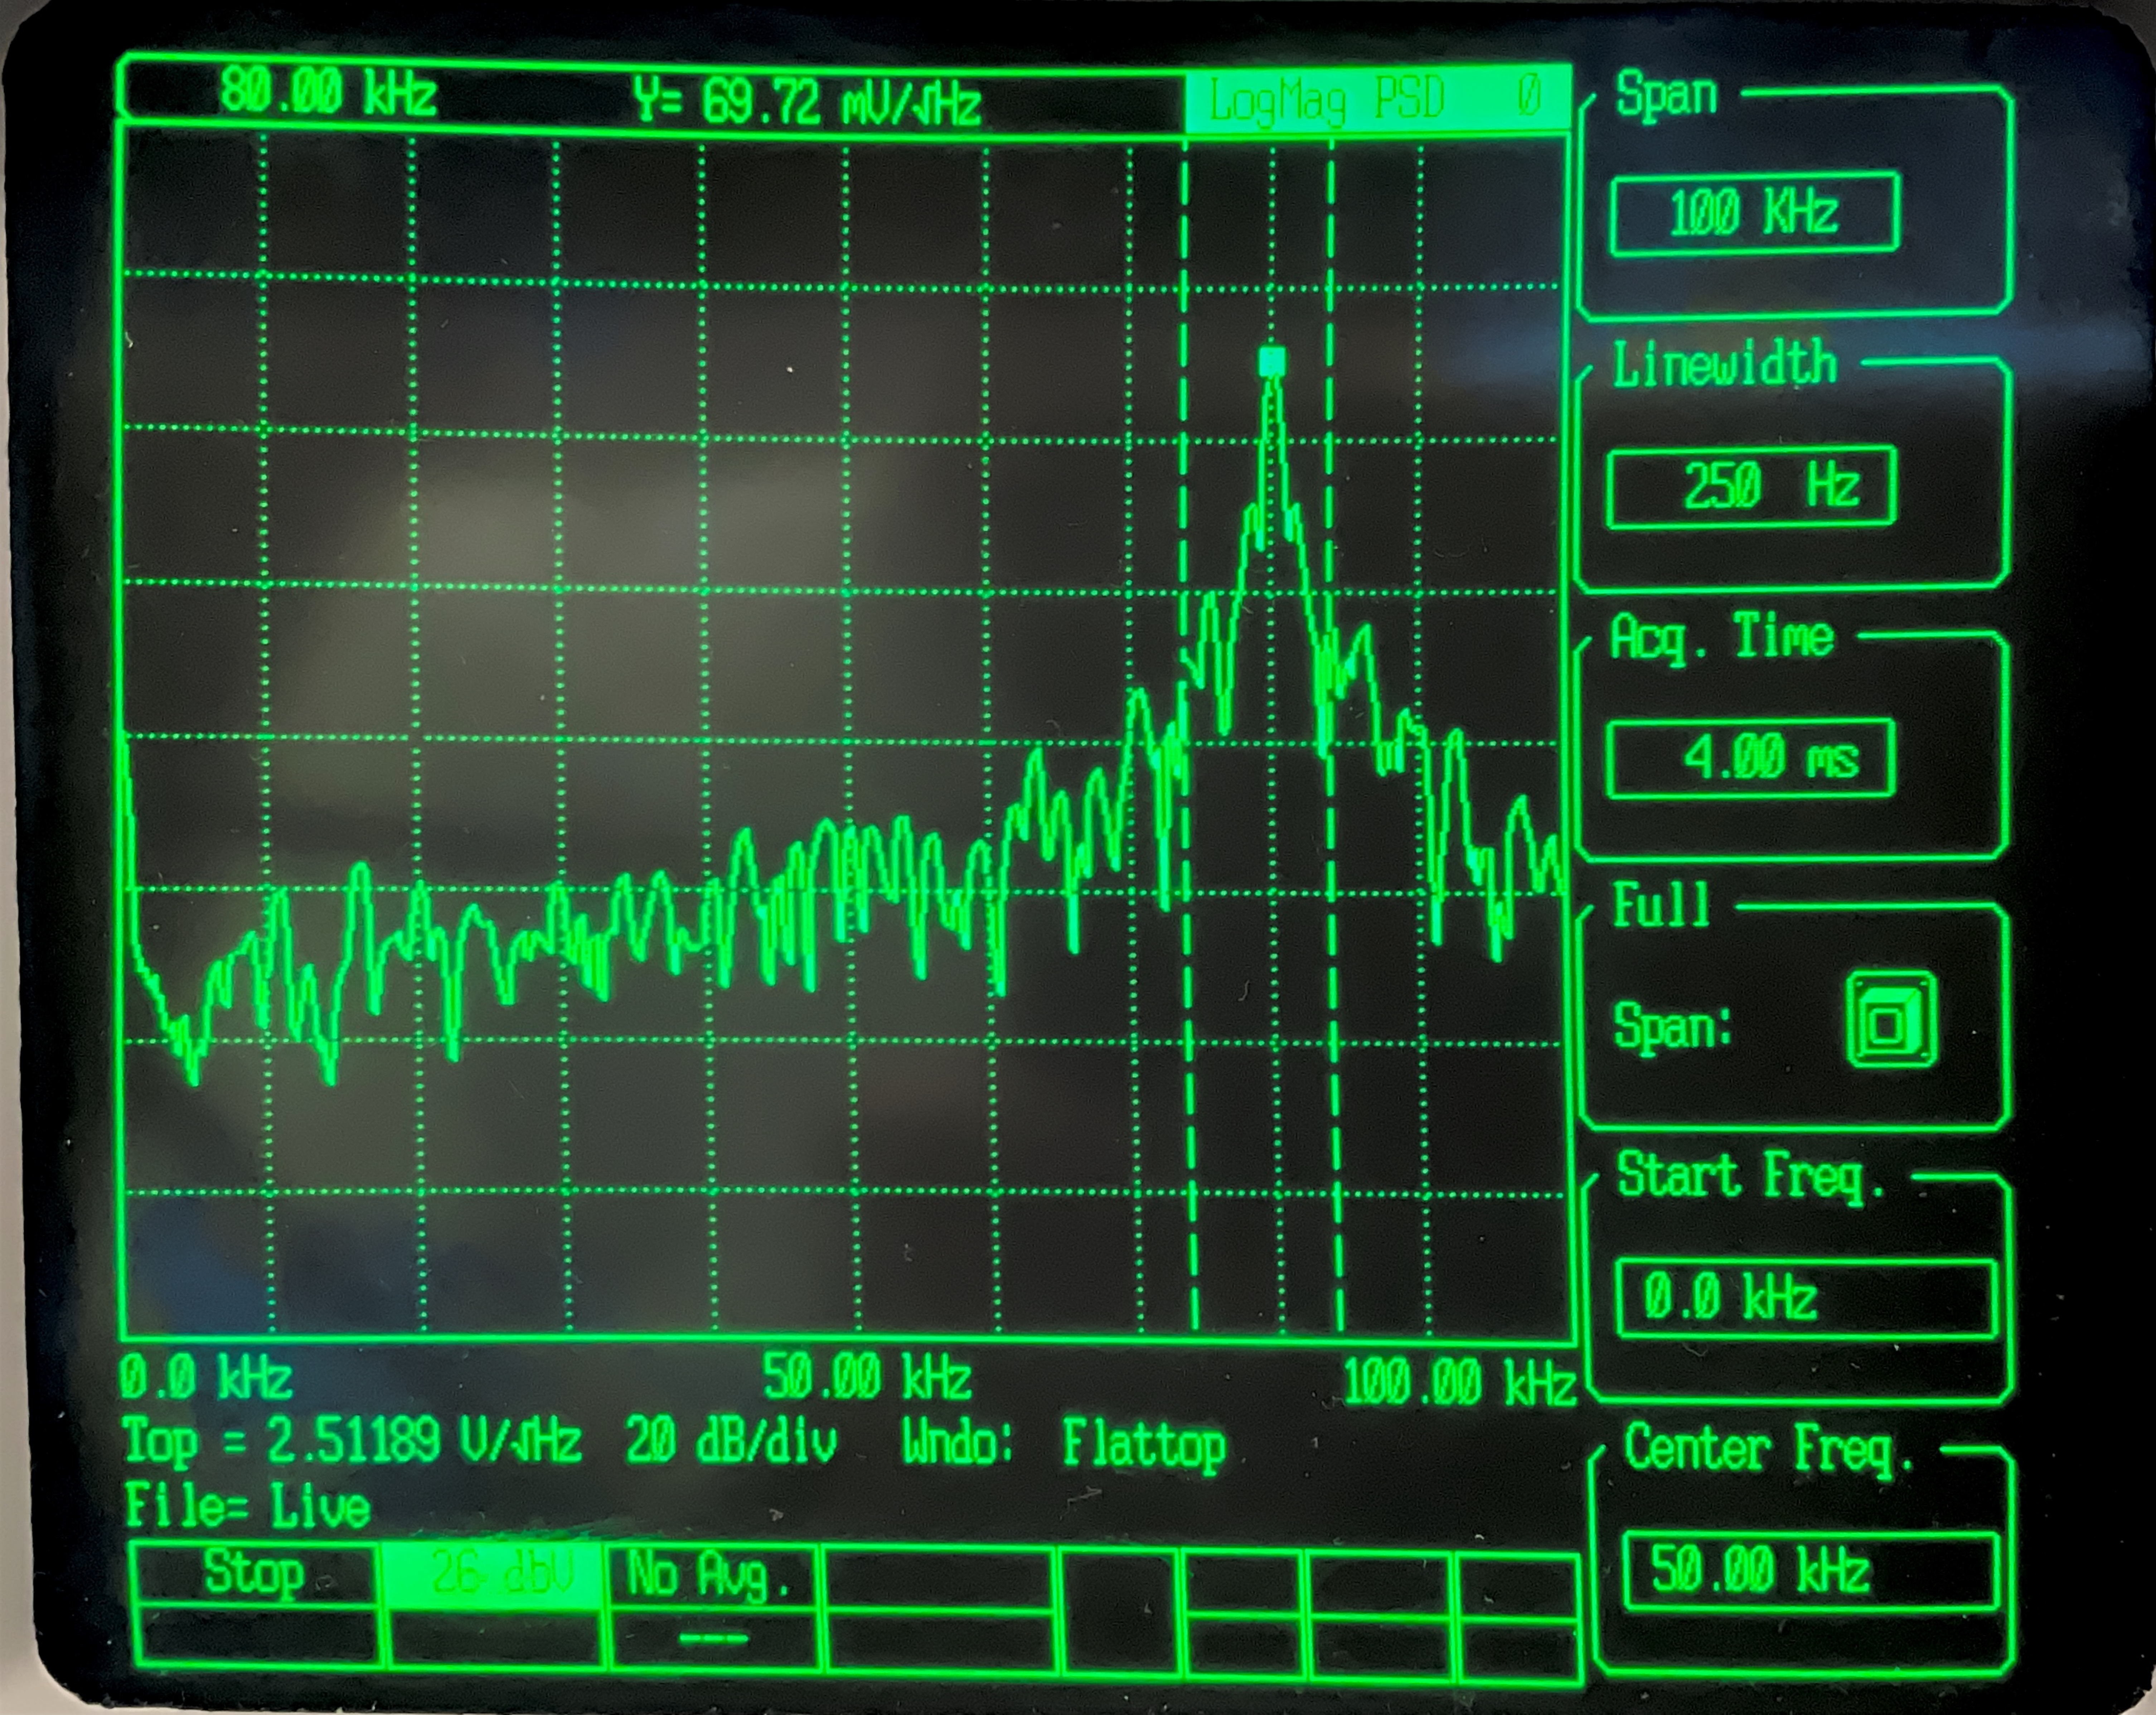
\includegraphics[width=\textwidth, page=1]{fig2_12.pdf}
        \caption{SR770 FFT Network Analyzer view}
        \label{fig:2.12b}
    \end{minipage}
\end{figure*}
Fig. \ref{fig:2.12} and \ref{fig:2.12b} show the oscilloscope and 770 view of the AM radio signal from KFUO 850 kHz 

\begin{itemize}
    \item In the down-conversion step, there is still mostly noise output (and some semblance of program content) from the speaker due to the wide band of the Filter module and the program content being downconverted to the wrong frequency of the original audio signal from the source.
    \item There are two choices for each difference frequency---e.g. $LO = RF \pm 80$ kHz.
    \newpage 
    \item Changing the LO frequency moves the large amplitude carrier frequency (and its program content) to the or right on the 770 i.e. the target RF frequency will be downconverted to a lower frequency $f_c = f_{RF} - f_{LO} = 850 - 800 = 50$ kHz as shown in Fig. \ref{fig:2.13}.
    % fig2_13.pdf
    \begin{figure}[ht]
        \centering
        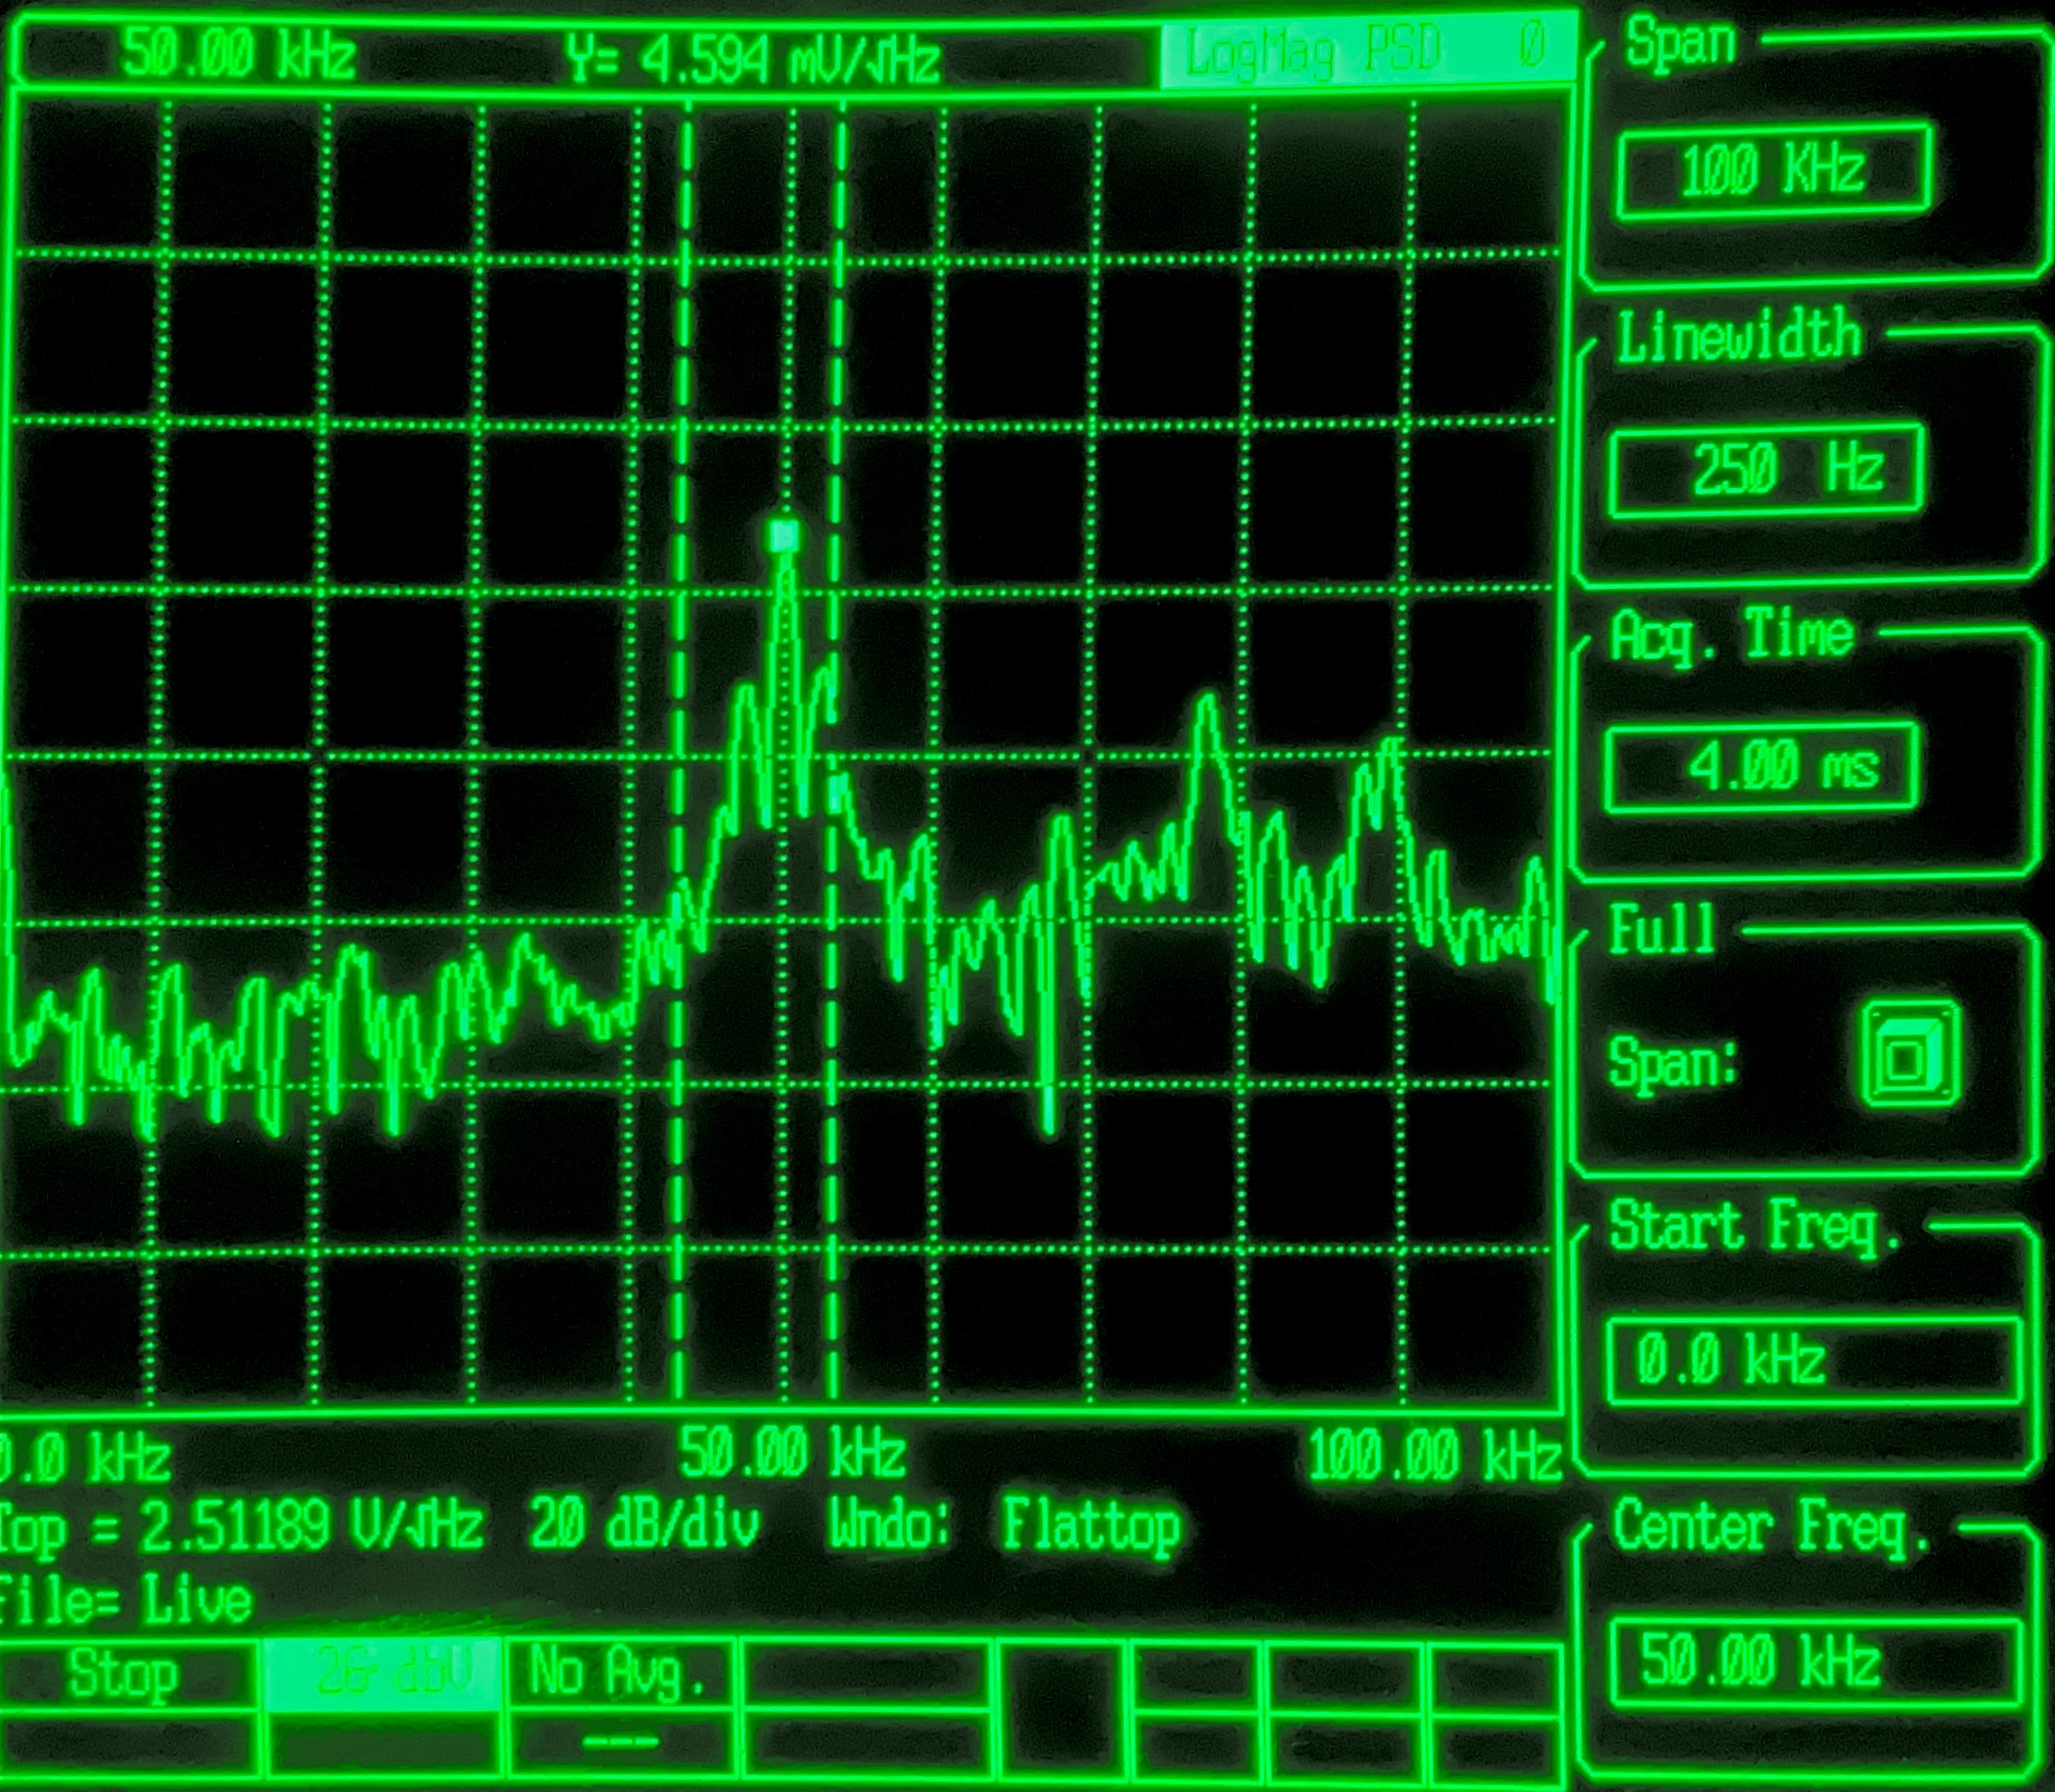
\includegraphics[width=0.45\textwidth]{fig2_13.pdf}
        \caption{Increasing LO frequency.}
        \label{fig:2.13}
    \end{figure}
    \item Thus de-modulating the signal by tuning the LO frequency to the carrier frequency $f_c  = f_{RF} - f_{LO} = 0$ will create a zero beat frequency and the sidebands of the IF will be the program content---i.e.
    an original audio signal (program content) $f_p$ from the source station is now correctly downconverted by the HF Mixer on the 770 as shown in Fig. \ref{fig:2.14}. 
    % fig2_14.pdf two pages
    \begin{figure*}[ht]
        \centering
        \begin{minipage}{0.45\textwidth}
            \centering
            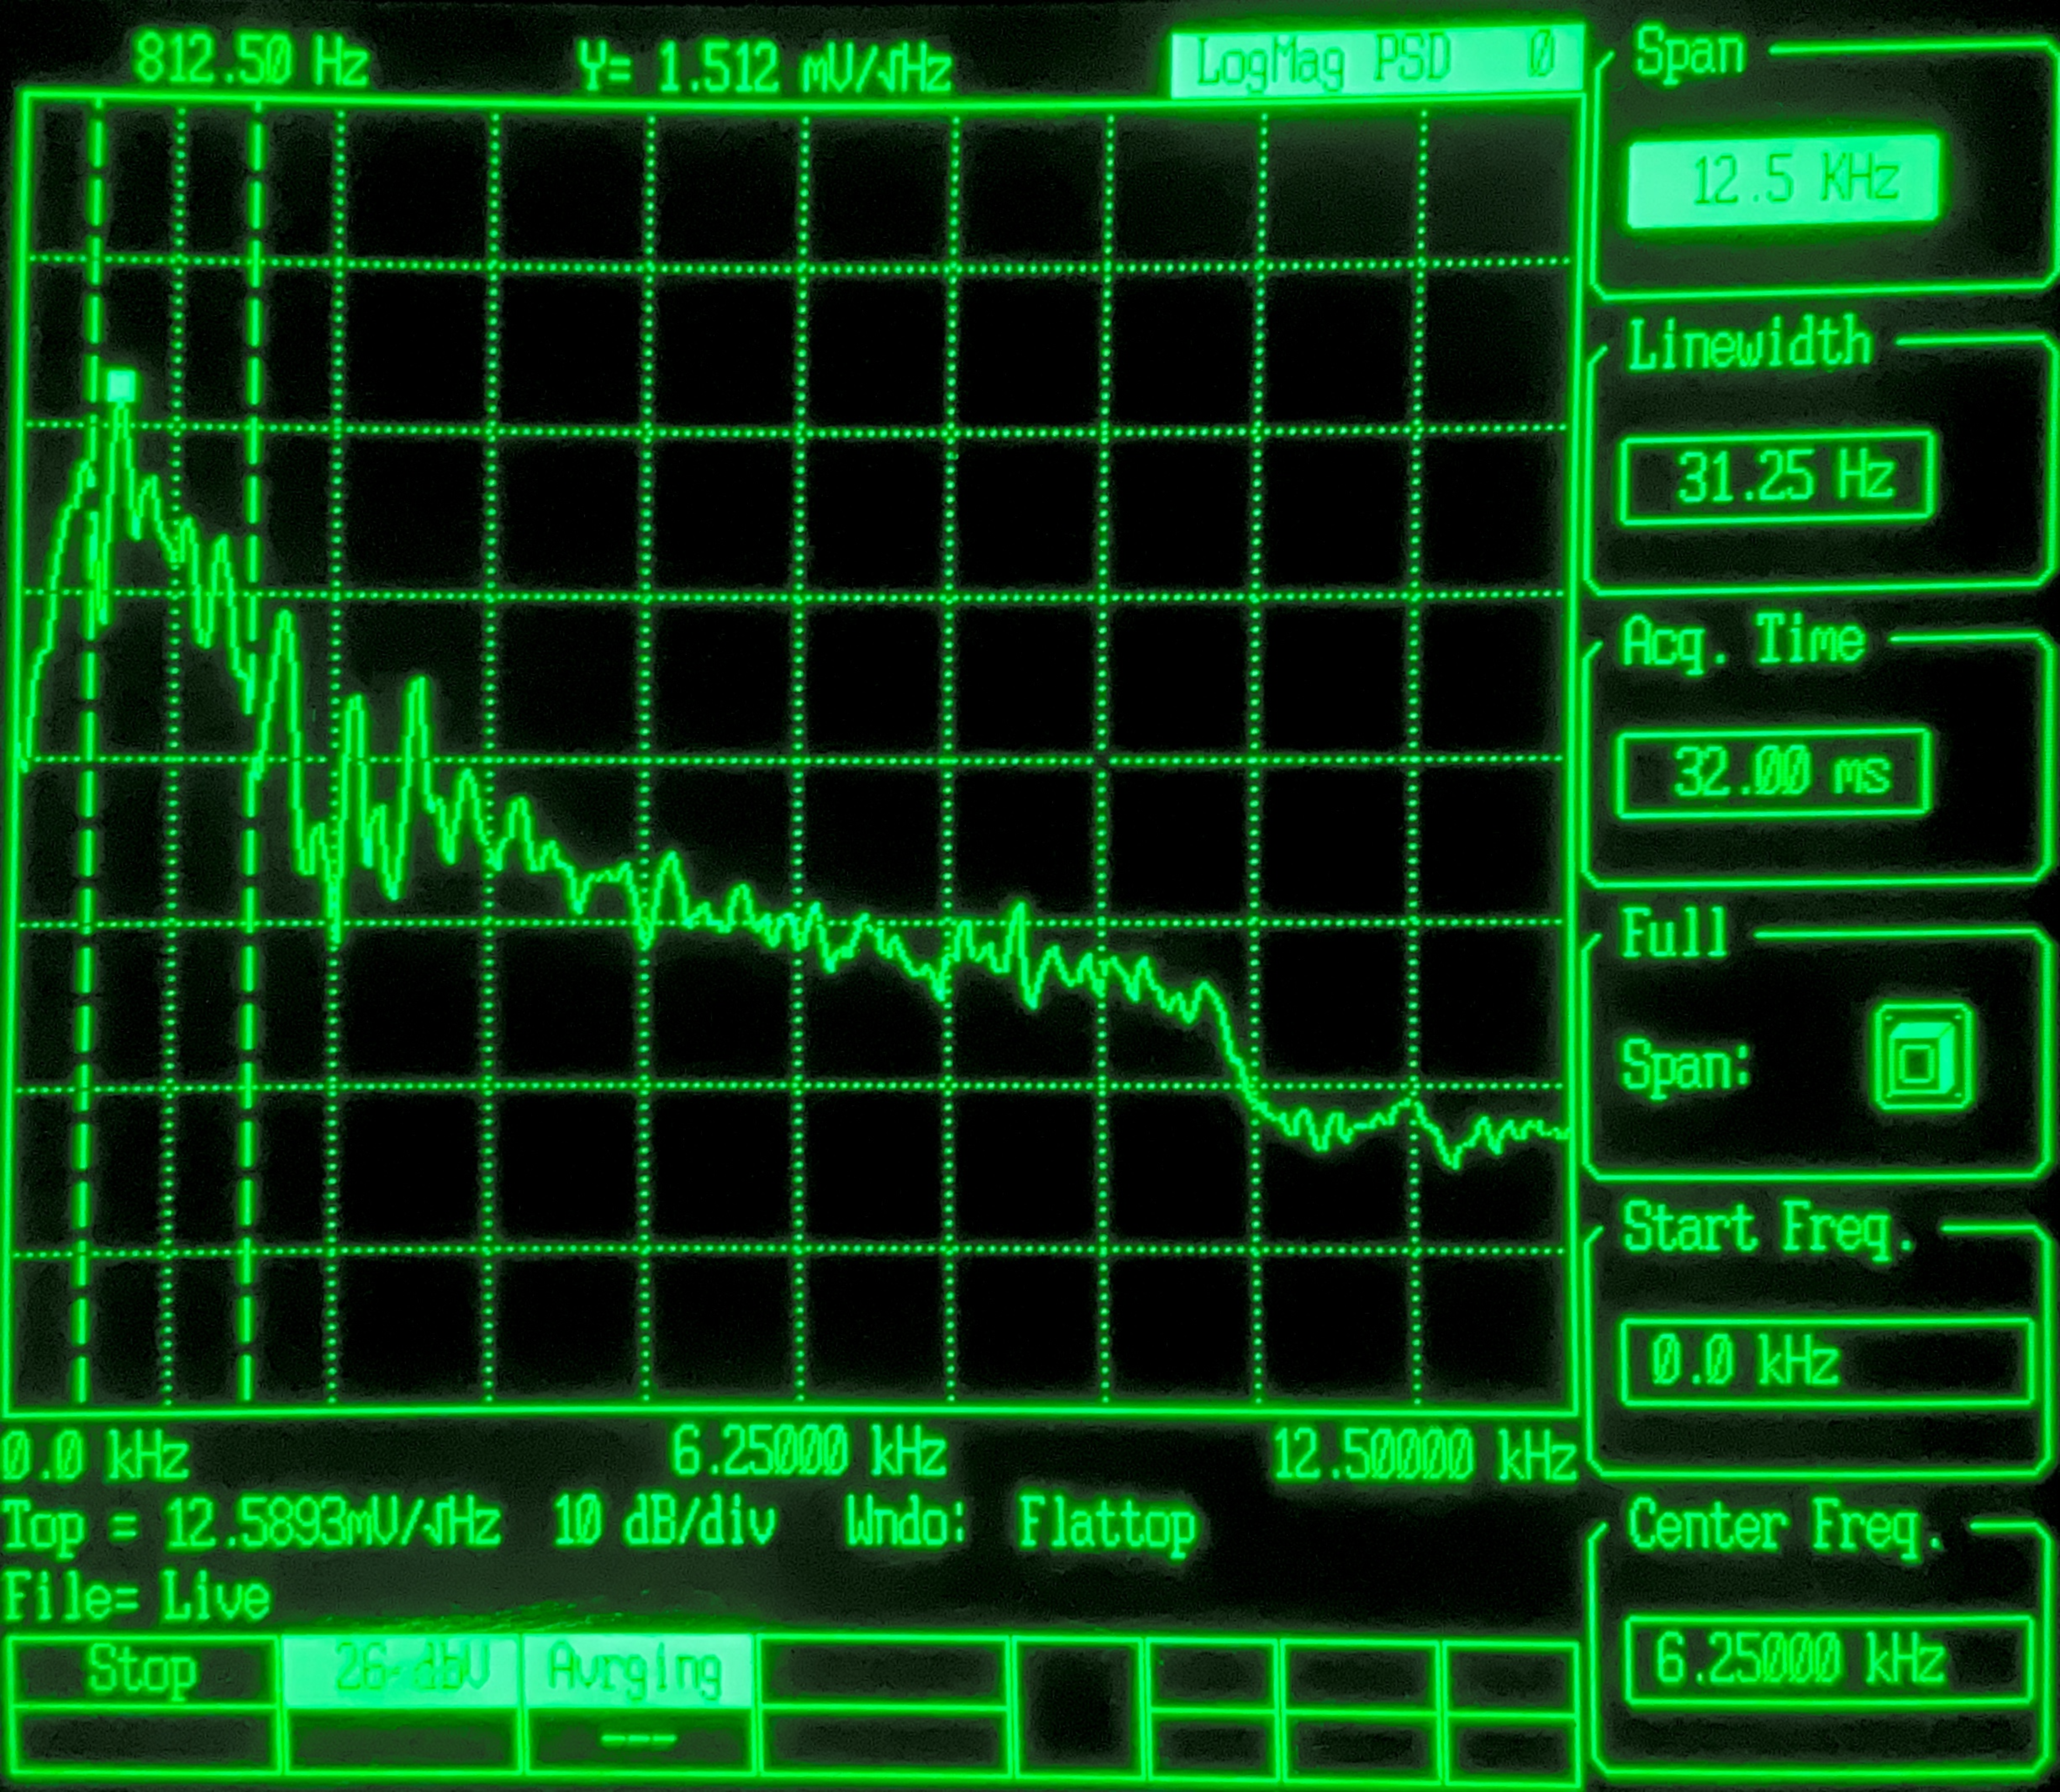
\includegraphics[width=\textwidth, page=1]{fig2_14.pdf}
            \caption{De-modulated signal at span of program content. The speaker outputs a sound of a piano and the 770 captures the frequency spectrum of the piano sound (with some noise).}
            \label{fig:2.14}
        \end{minipage}\hfill
        \begin{minipage}{0.45\textwidth}
            \centering
            \includegraphics[width=\textwidth, page=2]{fig2_14.pdf}
            \caption{De-modulated signal in full span view}
            \label{fig:2.14b}
        \end{minipage}
    \end{figure*}
    Furthermore, when a speaker is talking on the radio station, the 770 captures the frequency spectrum of the human voice in real time showing the resonant frequencies of the human voice (Fig. \ref{fig:2.15}).
    % fig2_15.pdf and fig2_16.pdf
    \begin{figure*}[ht]
        \centering
        \begin{tabular}{cc}
            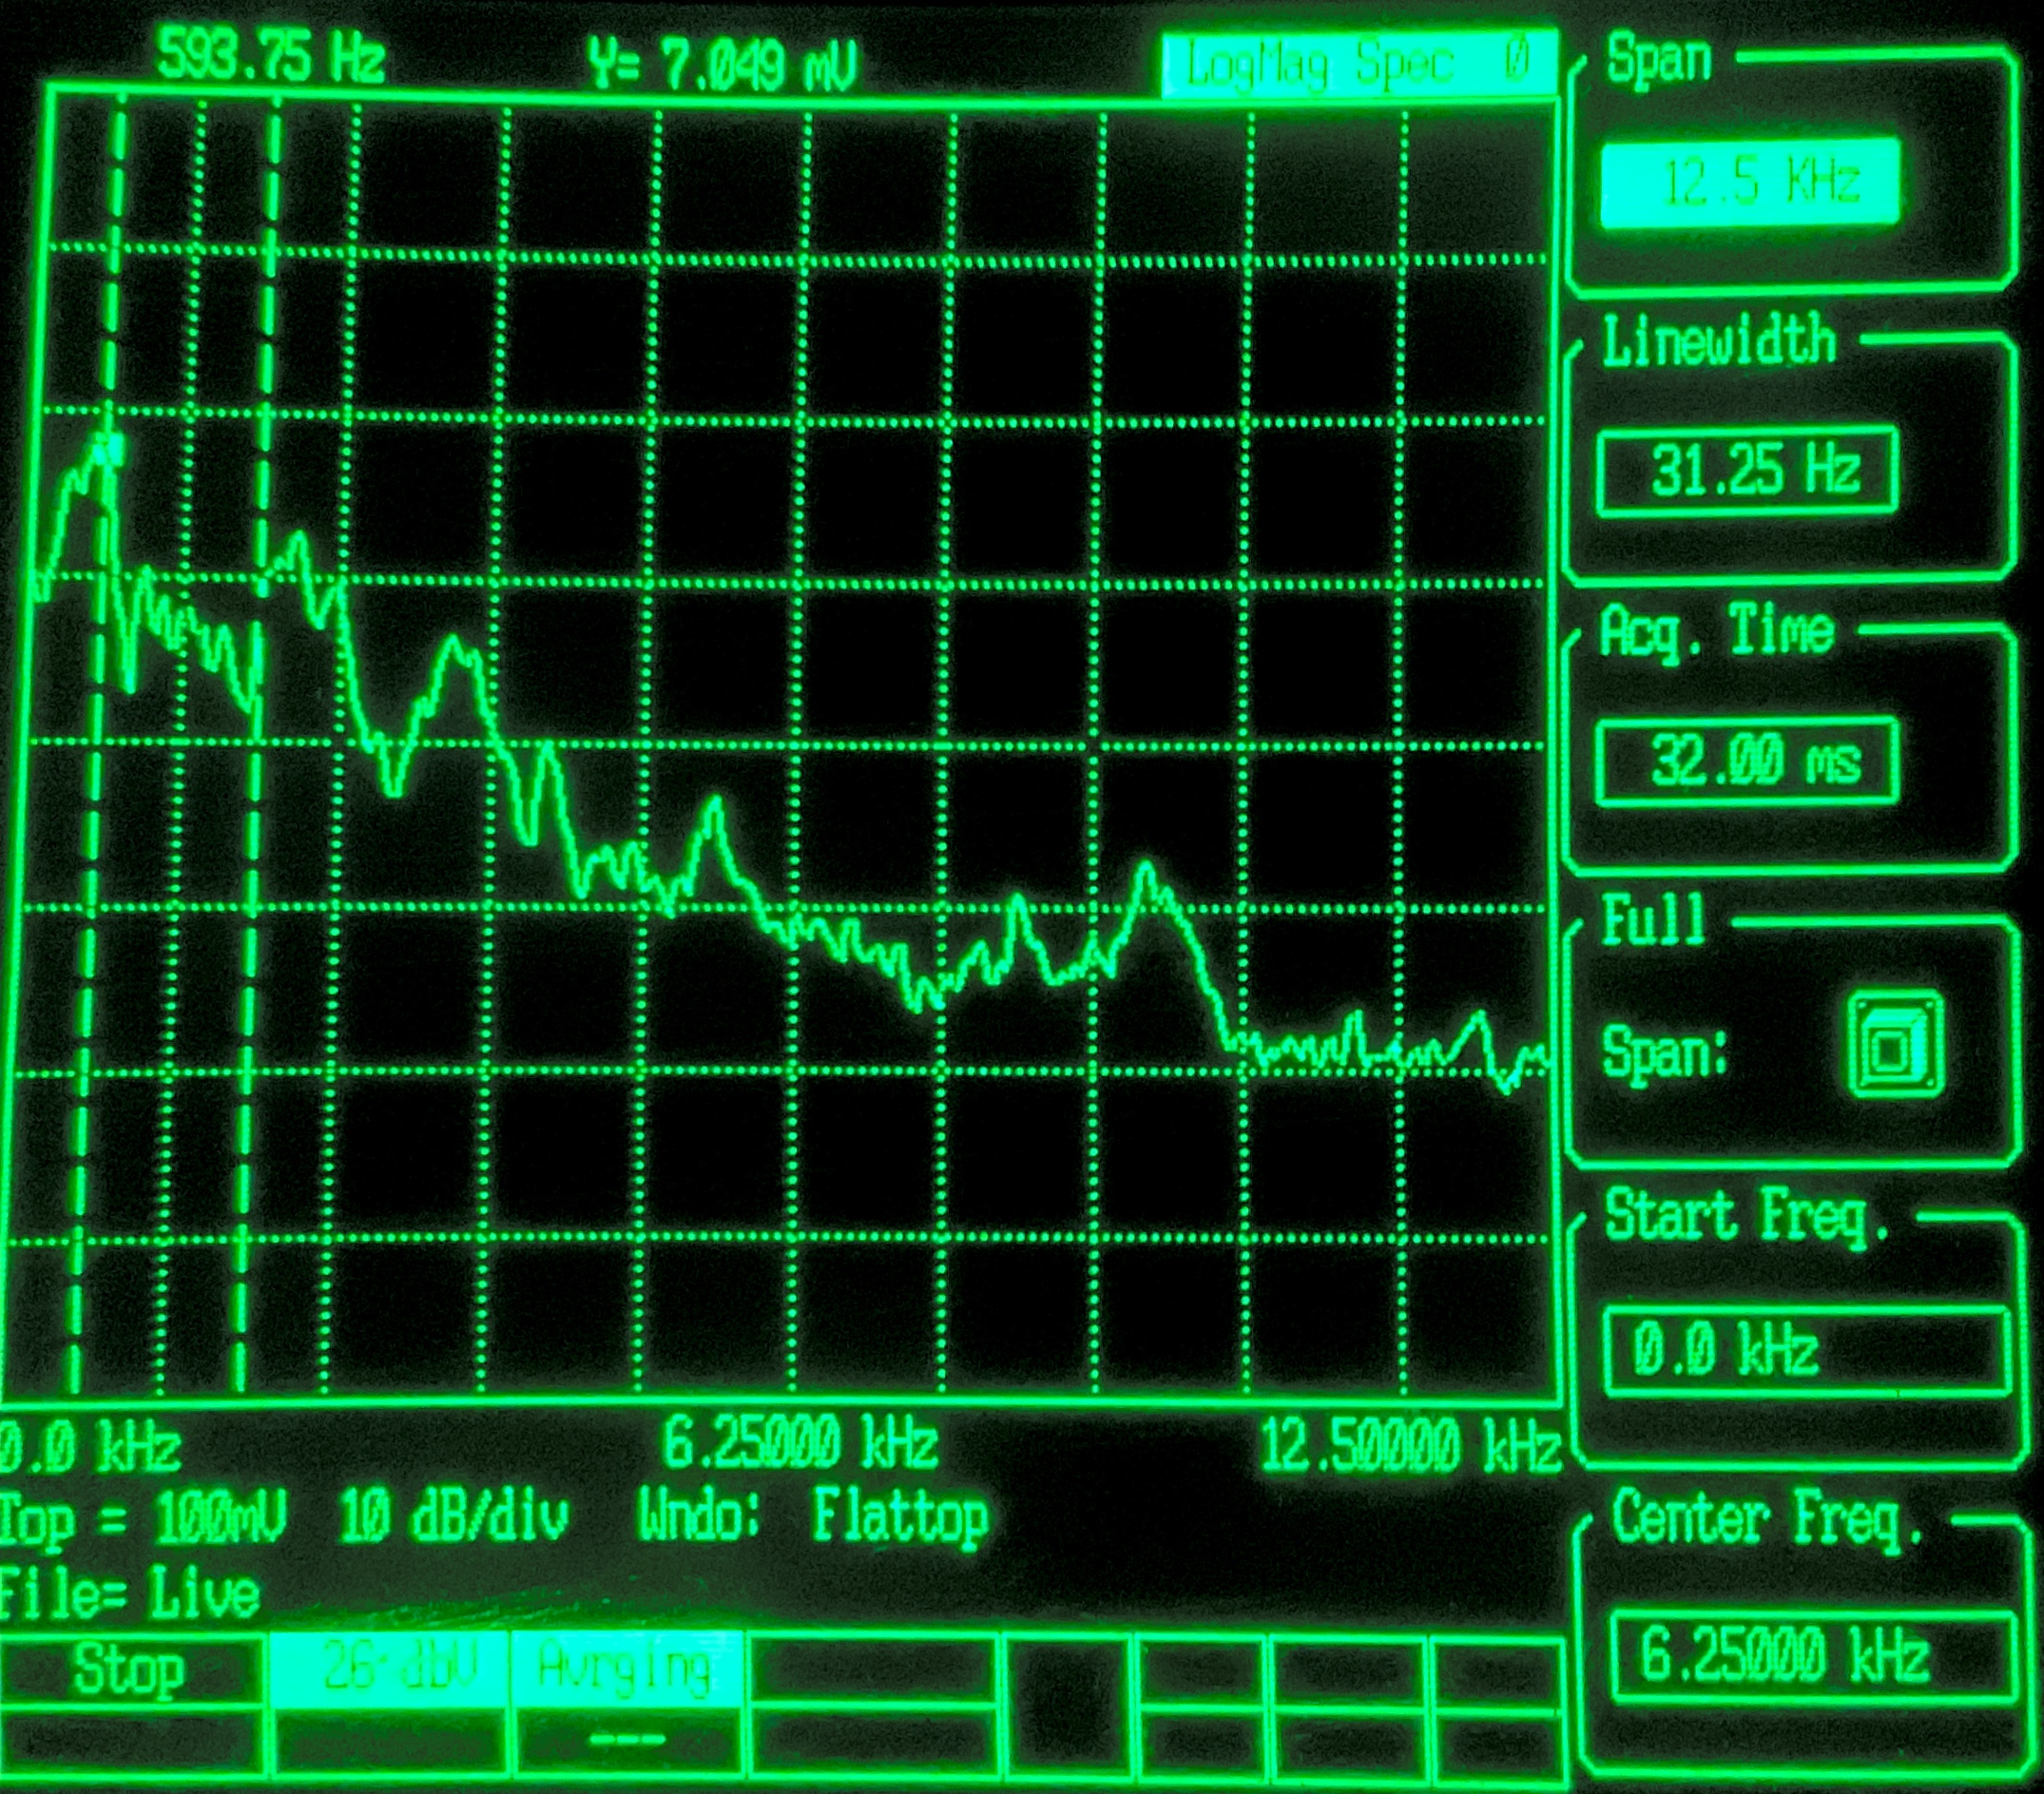
\includegraphics[width=0.45\textwidth]{fig2_15.pdf} & 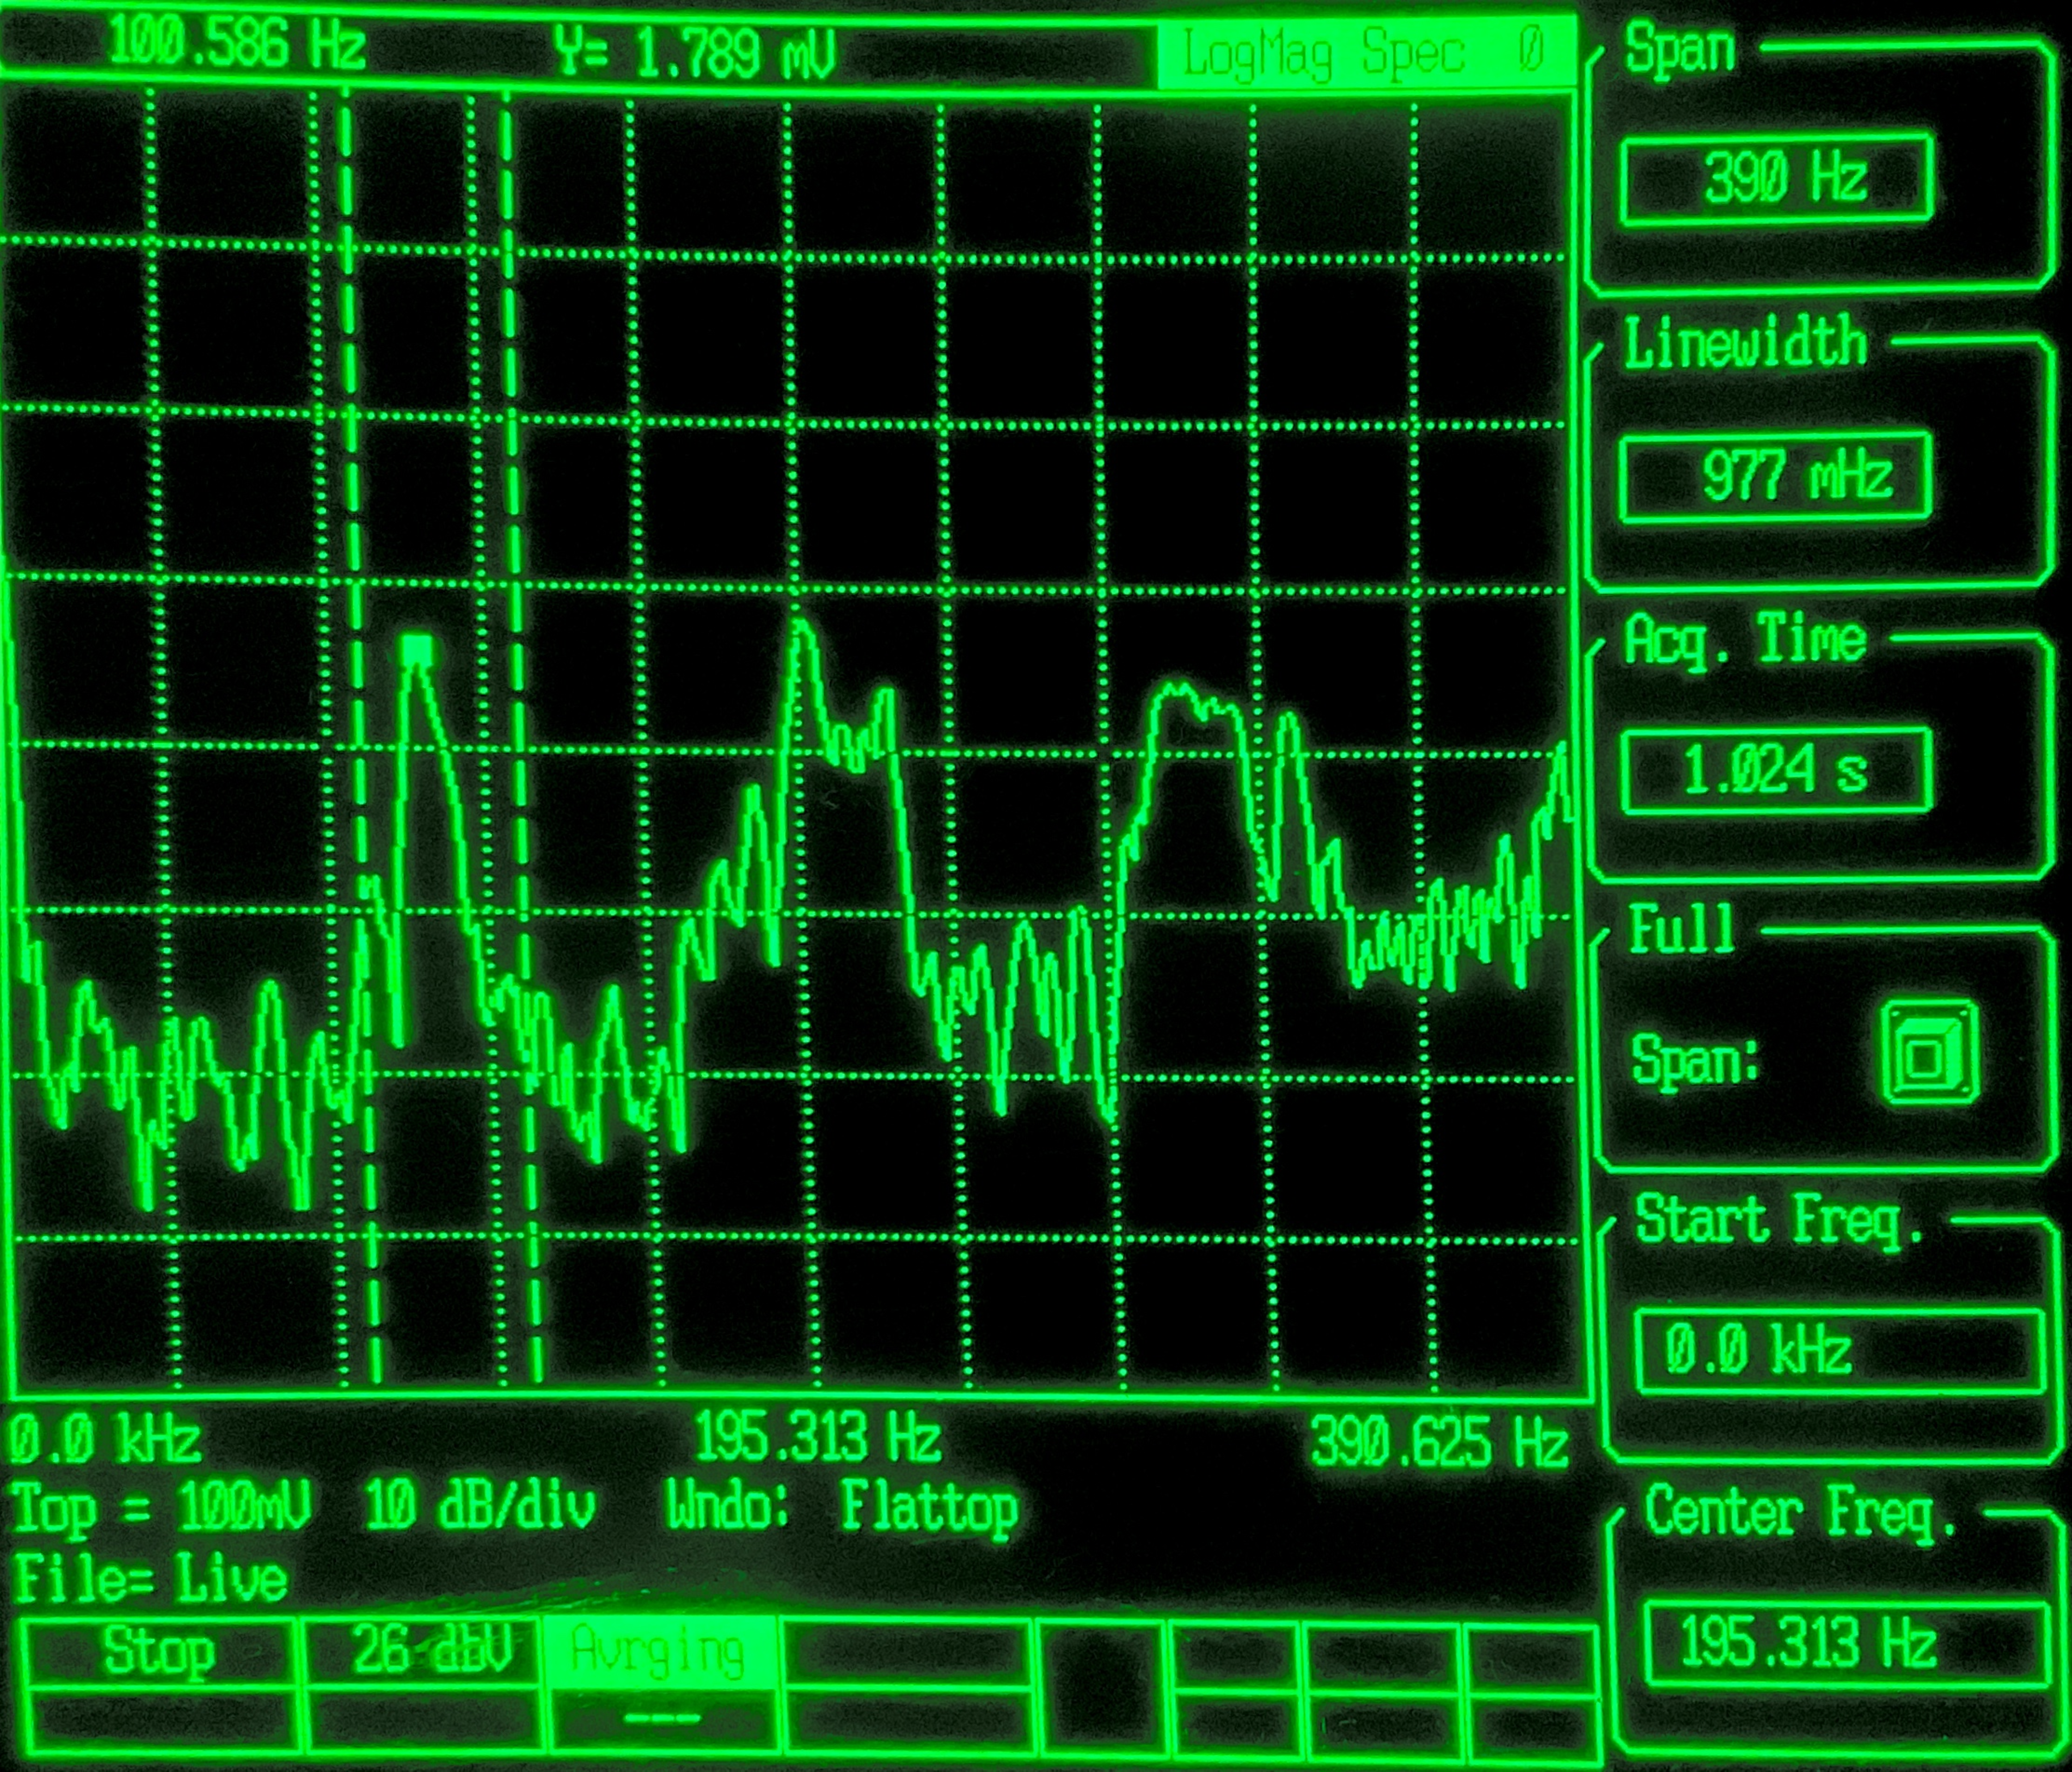
\includegraphics[width=0.45\textwidth]{fig2_16.pdf}
        \end{tabular}
        \captionsetup{width=0.8\textwidth}
        \caption{Snapshot of De-modulated signal of a human radio voice. 12 kHz span (left) shows high resonant frequencies (Formant) and 390 kHz span (right) shows the lower fundamental frequency (this is a different snapshot of the Radio voice since we can't capture two frequency ranges simultaneously) }
        \label{fig:2.15}
    \end{figure*}

    \newpage
    The 770 shows, in addition to the fundamental frequency of the human voice, there are high resonant frequencies present in certain vowels (formants);
    e.g. we can see formants $F_1 = 500$ Hz (fundamental frequency), $F_2 = 2.13$ kHz, $F_3 = 3.375$ kHz in Fig. \ref{fig:2.15} which are characteristic of the human voice.

    Source: ``Static measurements of vowel formant frequencies and bandwidths: A review'', Raymond D. Kent, Houri Vorperian \href{https://www.sciencedirect.com/science/article/pii/S0021992417302575}{(link)}
    
    doi: https://doi.org/10.1016/j.jcomdis.2018.05.004
\end{itemize}

\subsubsection*{Summary}

\begin{itemize}
    \item AM Modulation: Heterodying (Down-conversion and demodulation) can be used to anaylze high frequency AM signals at low frequency ranges and extract the program content of a radio station.
    \item Further applications: Formants to identify human speech and other audio signals (first step in speech recognition).

    Source: ``Formant estimation for speech recognition'', L. Welling, H. Ney (1998) \href{https://ieeexplore.ieee.org/abstract/document/650308}{link}

    doi: https://doi.org/10.1109/89.650308
\end{itemize}
\end{document}